\documentclass{VUMIFPSbakalaurinis}
\usepackage{algorithmicx}
\usepackage{algorithm}
\usepackage{algpseudocode}
\usepackage{amsfonts}
\usepackage{amsmath}
\usepackage{bm}
\usepackage{caption}
\usepackage{color}
\usepackage{float}
\usepackage{graphicx}
\usepackage{listings}
\usepackage{subfig}
\usepackage{wrapfig}

\usepackage{color}
\definecolor{todo-background-color}{rgb}{0.7, 0.7, 0.7}
\newcommand{\TODO}[1]{
\colorbox{todo-background-color}{TODO: #1}
}


% Titulinio aprašas
\university{Vilniaus universitetas}
\faculty{Matematikos ir informatikos fakultetas}
\department{Programų sistemų katedra}
\papertype{Bakalauro baigiamasis darbas}
\title{Duomenų dimensiškumo mažinimas ir klasifikavimas}
\titleineng{Dimensionality reduction and classification}
\author{Donatas Kučinskas}
\supervisor{lekt. Vytautas Valaitis}
\reviewer{asist. Julija Vysockytė}
\date{Vilnius – \the\year}

% Nustatymai
\setmainfont{Palemonas}   % Pakeisti teksto šriftą į Palemonas (turi būti įdiegtas sistemoje)
\bibliography{bibliografija}


\usepackage{caption}
\captionsetup[figure]{labelsep=space}


%\usepackage{titlesec}
%\titleformat{\section}[block]{\Large\fontsize{14}{14}\bfseries\filcenter}{}{1em}{}

% 14?


\begin{document}

\maketitle

\setcounter{page}{2}
% Padėkų skyrius
% \sectionnonumnocontent{}
% \vspace{7cm}
% \begin{center}
%     Padėkos asmenims ir/ar organizacijoms
% \end{center}



\sectionnonumnocontent{Santrauka}
% Glaustai aprašomas darbo turinys: pristatoma nagrinėta problema ir padarytos išvados.
% Santraukos apimtis ne didesnė nei 0,5 puslapio.

Darbe nagrinėjama klasifikavimo problema.
Tiriama, kaip galima pagerinti klasifikavimo rezultatus, mažinant klasifikuojamų duomenų dimensiškumą.
Klasifikavimas bei dimensiškumo mažinimas atliekami naudojantis atitinkamais daugiasluoksniais perceptronais.
Tyrimui naudojami didelio dimensiškumo biomedicinos duomenys.

% dimensiškumo mažinimas
Tiriama, kaip dimensiškumo mažinimas įtakoja duomenų savybių praradimą.
Atrasta, kad mažinant dimensijų skaičių, iki tam tikros ribos informacija beveik neprarandama, tačiau toliau mažinant dimensijų skaičių, prarandama informacijos dalis pradeda stipriai didėti.
Tiriamos daugiasluoksnio perceptrono galimybės išmokti sumažinto dimensiškumo duomenis nenaudojant validacijos grupės.
Atrasta, kad tinklas geba išmokti duomenis tol, kol dimensijų skaičius siekia bent 6 - su mažesniais dimensijų skaičiais dėl per didelio prarasto informacijos kiekio tinklas net nebegali pakankamai gerai išmokti mokymo duomenų rinkinio.

% klasifikavimo rezultatai
Taip pat buvo ištirti klasifikavimo rezultatai su originaliais bei sumažinto dimensiškumo duomenimis.
Nustatyta, kad dimensijų skaičių sumažinus iki daugumos intervalo $[14; 29]$ skaičių, pasiekiami geresni klasifikavimo rezultatai.
Vieni geriausių rezultatų pasiekiami su 18 dimensijų.
Šių duomenų klasifikavimas palygintas su nemažinto dimensiškumo duomenimis - gauti rezultatai, parodantys klasifikavimo rezultatų pagerėjimą.

% klasifikavimo palyginimas su 18-D
%Nemažinto dimensiškumo duomenų klasifikavimas buvo palygintas su duomenų, kurių dimensijų skaičius buvo sumažintas iki 18.
% Abiem atvejais tinklas mokymo duomenys buvo tinkamai įsisavinti, kadangi mokymo klaidos beveik pasiekė nulines.
% Visgi klasifikavimą geriau perprato ..., kadangi su šiais duomenimis validacijos klaida buvo pasiekta mažesnė.

% Dažniausiai toks dimensiškumo mažinimas naudojamas išskirti daug dimensijų turinčių duomenų bruožus.
% Tyrimui buvo naudojami biomedicinos duomenys, kadangi juose yra pakankamai dimensijų - kiekviena chromosoma aprašoma 30-ia parametrų.
% Šie duomenys buvo klasifikuojami naudojant daugiasluoksnį perceptroną.


% Nurodomi iki 5 svarbiausių temos raktinių žodžių (terminų).

\raktiniaizodziai{diagiasluoksnis perceptronas, klasifikacija, daugiamačiai duomenys, dimensiškumo mažinimas}



\sectionnonumnocontent{Summary}

\TODO{summary}

\keywords{multilayer perceptron, classification, high-dimensional data, dimensionality reduction}








\tableofcontents



\sectionnonum{Įvadas}

% apibrėžiamas tiriamasis objektas akcentuojant neapibrėžtumą, kuris bus išspręstas darbe,
% aptariamos teorinės darbo prielaidos bei metodika,
% apibūdinami su tema susiję literatūros ar kitokie šaltiniai, temos analizės tvarka, darbo atlikimo aplinkybės,
% Darbo įvadas neturi būti dėstymo santrauka

%tiriamas objektas - kompresijos rezultato gerinimas mažinant duomenų dimensiškumą


% 2-4 psl.


Klasifikavimas - tai dažnai sutinkama problema, turinti daugybę įvairių sprendimo būdų.
Ši problema labai dažnai sutinkama realybėje beveik visose srityse - medicinoje, genetikoje, ekonomikoje, sociologijoje, chemijoje ir daugybėje kitų.
Šio uždavinio tikslas - identifikuoti, kuriai grupei priklauso tiriamas objektas.
Tiriamieji objektai būna aprašomi tam tikrais parametrais, o grupės, kuriems jie yra priskiriami - iš anksto žinomos.
Pagal turimus objekto parametrus reikia nustatyti, kuriai grupei tikrinamasis objektas priklauso.

Norint išspręsti konkretų klasifikavimo uždavinį, akivaizdžiausias sprendimas galėtų būti šių grupių ištyrimas, analizuojant, kokiomis parametrų savybėmis pasižymi kiekvienos grupės objektai.
Tačiau problema kyla, kai tiriamų objektų klasės yra labai panašios viena į kitą - tokiu atveju pastebėti tam tikrus klasių skirtumus ir dėsningumus bei juos sumodeliuoti ir realizuoti yra kur kas sunkiau.
Be to, sprendžiant konkretų klasifikavimo uždavinį, tektų analizuoti klasifikuojamus objektus, o tam reikėtų ne tik gilių žinių apie šiuos objektus, bet ir daug pastangų.
Dažniausiai įvairūs dėsningumai apima ne vieną dydį, bet jų kombinaciją, kurią atrasti ir apskaičiuoti nėra lengva.
O norint efektyviai atskirti tam tikras objektų klases, gali prireikti daugybės skirtingų dėsningumų.
Šios priežastys labai apsunkina efektyvaus klasifikavimo algoritmo kūrimą analizuojant klases, todėl dažniau yra taikomi bendresni klasifikavimo sprendimai.

Vienas populiariausių klasifikavimo sprendimo metodų - klasifikavimas naudojant daugiasluoksnį perceptroną.
Turint pakankamai didelį tiriamų objektų duomenų kiekį, galima aptikti tam tikrus dėsningumus, kuriais skirtingų grupių objektai išsiskiria.
Šis metodas leidžia tai automatizuoti - vietoje to, kad žmogus mokytųsi apie objekto savybes ir jas analizuotų, tai atliekama naudojantis daugiasluoksniu perceptronu.
Turimi duomenys panaudojami apmokant daugiasluoksnį perceptroną, kuris po to geba klasifikuoti - pateikus objekto parametrus, tinklas nurodo, kuriai grupei šis objektas priklauso.
Žinoma, šio tinklo pateikiami atsakymai nėra visada teisingi, kadangi jis remiasi patirtimi, kurią įgijo pavyzdinių duomenų apmokymo metu, tačiau jei apmokymui buvo panaudota pakankamai korektiškų duomenų, pateikiami atsakymai būna ganėtinai tikslūs.

Dažnai tenka klasifikuoti objektus, turinčius labai didelį parametrų skaičių.
Tai apsunkina klasifikavimą naudojantis daugiasluoksniu perceptronu.
Nagrinėjant tiriamuosius objektus kaip taškus $N$-matėje erdvėje, kur $N$ yra parametrų skaičius, galima suprasti, kad kuo dimensijų skaičius yra didesnis, tuo taškai, atitinkantys tiriamuosius objektus, turi daugiau laisvės erdvėje.
Realybėje apmokant klasifikavimo tinklą naudojamas baigtinis objektų skaičius, todėl kuo šių duomenų dimensiškumas didesnis, tuo šie taškai bus rečiau išsidėstę erdvėje, o tai apsunkina daugiasluoksnio perceptrono darbą.
Dėl to dažnai bandoma sumažinti klasifikavimo duomenų dimensiškumą.

Dimensiškumo mažinimui taip pat yra aprašyta daugybė skirtingų sprendimo metodikų.
Dalis jų remiasi statistine duomenų analize, tyrinėjant turimų duomenų parametrų reikšmes, jų tarpusavio priklausomybes.
Kiti metodai naudojasi daugiasluoksniu perceptronu, mokydamiesi mažinti duomenų dimensiškumą.
Taip pat kai kurie metodai išnaudoja informaciją apie objektų klases - mažina duomenų dimensiškumą atsižvelgdami į skirtingų grupių parametrų savybes.
Darbe nagrinėjami keli populiariausi dimensiškumo mažinimo metodai.

Šio darbo tikslas - ištirti, ar galima ir kaip stipriai galima pagerinti klasifikavimą sumažinant klasifikavimui naudojamų duomenų dimensiškumą.

Darbo uždaviniai:
\begin{enumerate}
	\item Suprogramuoti daugiasluoksnį perceptroną.
	\item Sukurti klasifikuojantį daugiasluoksnį perceptroną.
	\item Parinkus tinkamus duomenis, ištestuoti klasifikuojantį daugiasluoksnį perceptroną.

	\item Ištirti dimensiškumo mažinimo metodus.
	\item Pasirinkti tyrimui tinkamą dimensiškumo mažinimo metodą.
	\item Realizuoti pasirinktą dimensiškumo mažinimo metodą.
	\item Ištirti dimensiškumo mažinimo įtaką duomenims.
	
	\item Ištirti, kaip keičiasi klasifikavimo rezultatas mažinant daugiasluoksniui perceptronui perduodamų duomenų dimensiškumą.
	\item Pasirinkti optimalų dimensijų skaičių, naudojamą dimensiškumo mažinimui.
	\item Palyginti daugiasluoksnių perceptronų apmokymo bei validacijos klaidas naudojant sumažinto ir nesumažinto dimensiškumo duomenis.
	\item Palyginti sumažinto ir nesumažinto dimensiškumo duomenų klasifikavimo rezultatus.
\end{enumerate}

Tyrimui naudojami chromosomų duomenys, panaudoti \cite[289~psl.]{price-dimensionality-reduction} tyrime.
Juos sudaro 12000 chromosomų, turinčių po 30 parametrų.
Šie duomenys leidžia efektyviai ištirti, kokią įtaką klasifikavimui daro dimensiškumo mažinimas, kadangi parametrų skaičius yra ganėtinai didelis ir yra pakankamai daug chromosomų, kad būtų galima dalį duomenų naudoti daugiasluoksnio perceptrono apmokymui, o kitą dalį - tinklo teisingumo testavimui.

Daugiasluoksniai perceptronai sprendžia daugybę skirtingų problemų, tačiau dažniausiai kiekviena jų sprendžiama vis kitaip.
Projektuojant daugiasluoksnį perceptroną, labai svarbu tiriama problema ir konkretūs tiriami duomenys.
Nuo jų priklauso, kokios struktūros tinklas geriausiai sprendžia analizuojamą problemą, kokie tinklo apmokymo metodai tinkamiausi ir pan.
Dėl to projektuojant daugiasluoksnius perceptronus, labai svarbu eksperimentuoti su skirtingomis tinklo architektūromis, skirtingais tinklo parametrais ir naudojamais metodais.

Tyrimams atlikti naudojama Python programavimo kalba.
\textit{Numpy} paketas naudojamas įvairiems skaičiavimams ir matricų operacijoms atlikti - jis ne tik supaprastina šias operacijas, tačiau ir kur kas pagreitina jas, kadangi bibliotekos pagrindinės funkcijos parašytos kompiliuojama kalba.
Duomenų vizualizavimui naudojamas \textit{Matplotlib} paketas.
Programavimui naudojama \textit{JetBrains PyCharm} integruota kūrimo aplinka (angl.~\textit{integrated development environment}).



\section{Dirbtinių neuronų tinklas}

Dirbtinis neuronų tinklas - tai tarpusavyje susijungusių dirbtinių neuronų tinklas, kurio užduotis yra spręsti tam tikrą konkrečią užduotį.
Gavęs pradinius užduoties duomenis, dirbtinis neuronų tinklas juos apdoroja ir taip gaunamas tam tikras atsakymas.
Šis atsakymas nebūtinai turi būti teisingas - neuronų tinklai suprojektuoti taip, kad galėtų būti mokomi iš padarytų klaidų tam, kad kitą kartą gautų teisingesnį atsakymą.

\subsection{Dirbtinis neuronas}

Dirbinių neuronų tinklas sudarytas iš daugybės dirbtinių neuronų, todėl norint suprasti tinklą, reikia pradėti nuo vieno dirbtinio neurono.
Žmogaus smegenys sudarytos iš daugybės neuronų.
Dirbtinis neuronas - tai supaprastintas šių biologinių neuronų modelis.
Jo modelis pavaizduotas \ref{fig:neuron}~paveiksle.
Dirbtinio neurono veikimo principas gan paprastas - per kairėje esančias jungtis dirbtinis neuronas gauna signalus iš kitų dirbtinių neuronų - iš $k$-tosios jungties gaunamas $x_k$ dydžio signalas.
Šiuos signalus neuronas apjungia ir pertvarko, ir taip sugeneruojamas dirbtinio neurono išeinamasis signalas.
Šis išeinamasis signalas gali būti siunčiamas daugybei kitų neuronų - dešinėje esančios jungtys yra neurono išeinamojo signalo jungtys, kuriomis ir yra siunčiamas išeinamasis signalas.

\begin{figure}[h]
	\centering
	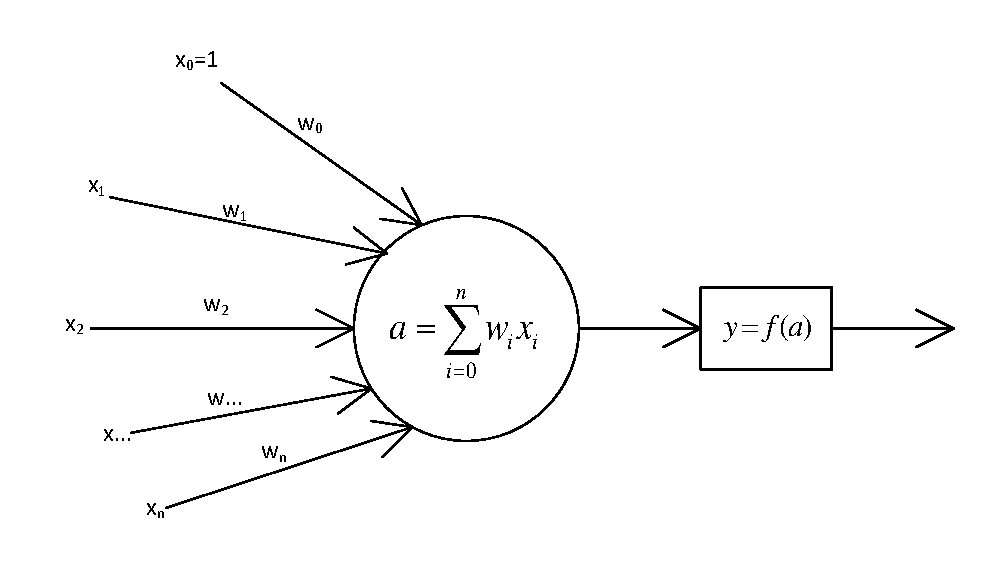
\includegraphics[scale=0.75]{diagrams/1_neuron}
	\caption{Dirbtinis neuronas}
	\label{fig:neuron}
\end{figure}

Dirbtinis neuronas generuoja išeinamąjį signalą pagal tam tikrą modelį.
Skaičiuojant neurono generuojamą signalą, kiekvienos įeinančiosios jungties $k$, turinčios svorį $w_k$ ir ja sklindantį signalą $x_k$ dydžio, šie du dydžiai yra sudauginami.
Tada visos šios signalų dydžių ir svorių sandaugos yra susumuojamos - taip gaunamas sužadinimo signalas $a$ (\ref{eq:a}~formulė).
Tada sužadinimo signalas $a$ yra paduodamas kaip argumentas tam tikrai funkcijai $f$ ir gaunamas neurono išeities signalas $y = f(a)$.
Šį funkcija $f$ yra vadinama aktyvacijos funkcija - ją galima pasirinkti pagal tai, kokio tikslo siekiama iš šio dirbtinio neurono.
Populiariausios aktyvacijos funkcijos - slenkstinė, tiesinė, hiperbolinis tangentas bei sigmoidinė, esanti \ref{eq:sigmoid}~formulėje.
Iš esmės aktyvacijos funkcija gali būti bet kokia funkcija, tačiau vėliau norint apmokyti dirbtinį neuronų tinklą, reikia rasti šios funkcijos išvestinę.
Dėl šios priežasties dažniausiai pasirenkamos tokios aktyvacijos funkcijos, kurios ne tik tinkamai pertvarko signalą išvedimui, tačiau ir kurios išvestinės yra paprastos.

\begin{equation} \label{eq:a}
a = \sum_{k=1}^N w_kx_k
\end{equation}

\begin{equation} \label{eq:sigmoid}
f(a) = \frac{1}{1 + e^{-a}}
\end{equation}

Įeinamosios neurono jungtys numeruojamos nuo 1 iki $k$.
Norint $a$ reikšmę padaryti tinkamesnę neuroninio tinklo funkcijoms, dažniausiai įvedama papildoma $0$-inė jungtis su svoriu $w_0$ ir signalo stiprumu $x_0 = 1$.
Tokiu būdu prie $a$ (\ref{eq:a}~formulė) reikšmės papildomai pridedama $w_0 * x_0 = w_0$ reikšmė.
Šis papildomas narys leidžia koreguoti neurono generuojamą signalą nepriklausomai nuo įeinančių jungčių signalų.



\subsection{Dirbtinių neuronų tinklas}

Dirbtinių neuronų tinklas (angl.~\textit{artificial neural network}) - tai tinklas, kurį sudaro dirbtiniai neuronai bei jungtys, jungiančios kai kuriuos dirbtinius neuronus.
Per kiekvieną jungtį gali eiti signalas, kuris perduoda vieno neurono išeinamąjį signalą kitam neuronui.
Kiekvienas neuronas gali turėti bet kokį skaičių įeinančių ir bet kokį skaičių išeinančių jungčių.

Kai kurios jungtys gali būti prijungtos tik prie vieno neurono.
Jungtys, kurios įeina į neuroną tačiau neišeina iš jokio neurono, gali būti naudojamos duomenų perdavimui - šiomis jungtimis neuronų tinklui perduodami signalai, atitinkantys duomenis.
Jungtys, išeinančios iš neurono tačiau neįeinančios į jokį neuroną, naudojamos rezultato gavimui - kai per visą neuroninį tinklą pereina signalai, būtent šiose jungtyse ir yra gaunamas pateiktus duomenis atitinkantis atsakymas.

Dirbtinio neuronų tinklo užduotis - pagal pateikiamus duomenis sugeneruoti atsakymą.
Pirmiausia duomenys pateikiami per tam skirtas jungtis.
Neuronai, prijungti prie šių jungčių, gauna šiuos pradinius signalus, juos apdoroja ir pradeda skleisti tam tikro stiprumo signalą išeinančiomis jungtimis.
Taip signalai sklinda tolyn ir visi tinklo neuronai būna apdorojami tol, kol galiausiai rezultatas būna gaunamas tam skirtose jungtyse.



\subsection{Daugiasluoksnis perceptronas}

Daugiasluoksnis perceptronas (angl.~\textit{multilayer perceptron}) - tai tam tikromis savybėmis pasižymintis dirbtinių neuronų tinklas.
Tai viena populiariausių dirbtinių neuroninių tinklų rūšis, kadangi savybės, kuriomis šis tinklas pasižymi, leidžia padaryti tam tikras skaičiavimo optimizacijas bei pakankamai lengvai realizuoti veikiantį neuroninį tinklą.
Be to, galima keisti daugiasluoksnio perceptrono parametrus pritaikant jį konkrečiai sprendžiamai problemai.

Neuronų tinklą galima nagrinėti kaip grafą, kuriame dirbtiniai neuronai yra grafo viršūnės, o jungtys, jungiančios juos - kryptinės grafo briaunos.
Jeigu neuronų tinklo grafe būtų bent vienas ciklas, tai reikštų, kad šiame cikle esančiomis jungtimis einantys signalai gali keistis ne kartą - atnaujinus tam tikro neurono išvedimo signalą, ciklu gali pakisti ir šio neurono įvedimo signalas.
Tada reikėtų vėl atnaujinti šio neurono išvedimo signalą, o tai darant vėl gali pasikeisti bet kuris įvedimo signalas ir toks pasikeitimų ciklas gali kartotis labai daug kartų arba net ir niekada nesibaigti.
Tai apsunkina dirbtinių neuronų veikimą, todėl dažniausiai naudojami neuronų tinklai, kuriais signalai skleidžiami pirmyn (angl.~\textit{feedforward}).
Pagal apibrėžimą, jeigu tinklo grafe nėra nei vieno ciklo, tinklas yra pirmyn skleidžiamas.

Tai, kad daugiasluoksnis perceptronas yra skleidžiamas pirmyn, suteikia nemažai privalumų.
Norint apdoroti tam tikrą neuroną, privalu žinoti visus įeinančiųjų jungčių signalų dydžius, o tai reiškia, kad jau turi būti apdoroti visi neuronai, kurių išeinamosios jungtys įeina į apdorojamąjį neuroną.
Grafe be ciklų rasti tokią neuronų seką, kuria būtų galima apdoroti tinklo neuronus nėra sunku - šį užduotis yra plačiai žinoma ir vadinama topologiniu rikiavimu.
Yra žinoma, kad beciklį grafą visada galima topologiškai išrikiuoti, o tai reiškia, kad daugiasluoksnį perceptroną galima apdoroti tiesiog paeiliui apdorojant topologiškai išrikiuotų viršūnių seką.
Šį savybė palengvina neuroninio tinklo apdorojimą.

Be to, daugiasluoksniai perceptronai yra organizuojami sluoksniais (žr. \ref{fig:neural_network} paveikslą).
Tinklas yra sudarytas iš perceptronų grupių, kurios yra vadinamos sluoksniais.
Visi neuronų sluoksniai yra išsidėstę iš eilės, nuo kairės į dešinę.
Kiekvieno sluoksnio visi neuronai turi išeinamąsias jungtis į visus neuronus iš sekančio sluoksnio, esančio dešinėje.
Išimtis paskutinis sluoksnis, vadinamas išvesties sluoksniu (angl.~\textit{output layer}) - kadangi jis naudojamas išvedimui, todėl neturi jungčių į kitus neuronus, o jo jungtyse formuojamas atsakymas į analizuojamą problemą.

\begin{figure}[h]
	\centering
	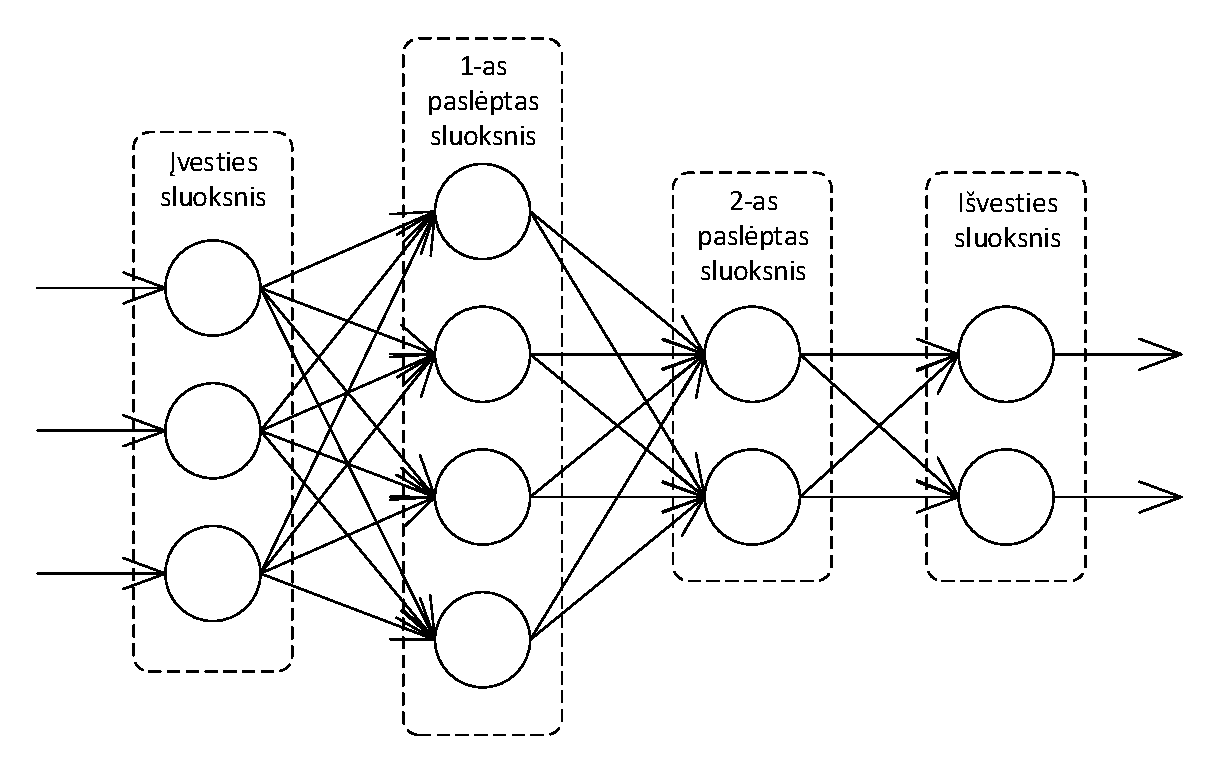
\includegraphics[scale=0.75]{diagrams/2_neural_network}
	\caption{Daugiasluoksnis perceptronas}
	\label{fig:neural_network}
\end{figure}

Pirmasis neuronų sluoksnis, kuriam paduodami duomenys, vadinamas įvesties sluoksniu (angl.~\textit{input layer}).
Po to gali būti vienas ar keli paslėpti sluoksniai (angl.~\textit{hidden layer}), kurie naudojami tam, kad neuroninio tinklo struktūra būtų didesnė ir gebėtų išmokti sudėtingesnius dalykus.
Paprasčiausiuose tinkluose gali išvis nebūti paslėptų sluoksnių, tačiau tokio tinklo galimybės būtų labai ribotos ir jo apmokymas sudėtingesnėms užduotims užtruktų daug ilgiau.
Paskutinysis sluoksnis, naudojamas rezultatų suformavimui, vadinamas išvesties sluoksniu.

Tokia neuronų organizacija į sluoksnius dar palengvina tinklo veikimą - signalus siųsti galima sluoksnis po sluoksnio, pradedant pirmuoju, kuris gauna problemos duomenis, siunčiant signalus visomis jungtimis antrajam sluoksniui.
Po to tas pats atliekama su antruoju sluoksniu siunčiant visus signalus trečiajam ir t.t., kol galiausiai rezultatai gaunami paskutiniame sluoksnyje.

Savybė, kad kiekvieno sluoksnio, išskyrus paskutinio, visi neuronai turi išeinamąsias jungtis į visus sekančio sluoksnio neuronus taip pat yra naudinga - žinant tai, nereikia turėti jokio tinklo grafo, kadangi užtenka žinoti kiekvieno sluoksnio neuronus bei jungčių svorius.
Be to, signalų siuntimas iš vieno sluoksnio į sekantį taip pat gali būti suprastintas.
Vietoj to, kad programiškai iteruoti per visas dviejų sluoksnių neuronų poras ir atlikti jungties dydžio skaičiavimą, tą galima padaryti su matricų aritmetika.
Signalo skaičiavimo atliekamas operacijas, nurodytas \ref{eq:a}~formulėje, galima sutraukti į matricų daugybos operacijas, o aktyvacijos funkciją pritaikyti visai matricai.
Taip daugiasluoksnio perceptrono tinklo modelis tampa dar tvarkingesnis ir paprastesnis.

Projektuojant daugiasluoksnį perceptroną konkrečiam uždaviniui, reikia parinkti jo struktūrą.
Reikia nuspręsti, kiek neuronų sluoksnių bus, kiek kiekviename sluoksnyje bus neuronų, kokios aktyvacijos funkcijos bus naudojamos, kaip duomenys yra paduodami, kokiu formatu iš tinklo gaunami rezultatai.
Norint efektyviai spręsti konkretų uždavinį, labai svarbu parinkti tinkamą struktūrą.
Nuo parinktos struktūros priklauso daugiasluoksnis perceptronas galimybės mokytis - parinkus blogą struktūrą, tinklas gali nesugebėti išmokti sudėtingesnių duomenų atvejų.



\subsection{Neuroninio tinklo apmokymas} \label{network-learning}

%Neuronų tinklo pateiktas atsakymas nebūtinai yra teisingas - neuronų tinklas suprojektuotas taip, kad jį būtų galima tobulinti pagal daromas klaidas.

Daugiasluoksnis perceptronas suprojektuotas taip, kad pagal mokymui naudojamus duomenis jis galėtų būti keičiamas ir jo pateikiami atsakymai panašėtų į teisingus.
%Pagal tinklo pateiktą rezultatą ir iš anksto žinomo rezultato skirtumus keičiami jungčių svoriai taip, kad kitą kartą būtų gaunamas atsakymas, artimesnis teisingam.
%Neuroniniui tinklui pateiktus neteisingą atsakymą, vykdomas tinklo mokymas.
Vienas populiariausių mokymo metodikų, kuri yra naudojamas šiame darbe - atgalinis propagavimas (angl.~\textit{backpropagation}).
Tam, kad būtų galima apmokyti neuronų tinklą spręsti konkrečią problemą, reikia turėti nemažą šios problemos pavyzdinių duomenų rinkinį bei iš anksto žinoti kiekvienų duomenų teisingą atsakymą.
Mokymas vyksta pažingsniui, vienu metu neuroniniui tinklui pateikiant vienus duomenis iš turimo duomenų rinkinio.
Neuroninis tinklas, gavęs duomenis, juos analizuoja ir pateikia tam tikrą atsakymą.
Šis gautas atsakymas yra sulyginamas su teisingu, iš anksto žinomu atsakymu.
Pagal tai, kaip neuroninio tinklo pateiktas atsakymas skiriasi nuo teisingojo, neuroninis tinklas būna pertvarkomas.
Pertvarkymas vyksta nagrinėjant neuroninį tinklą pradedant nuo paskutinio sluoksnio ir baigiant pirmuoju - t. y. priešinga tvarka, nei buvo nagrinėjama, kai neuroninis tinklas analizavo pateiktus duomenis.
Nagrinėjant kiekvieną neuroninio tinklo neuroną, į jį įeinančių jungčių svoriai $w_k$ (įskaitant ir $w_0$, kuris naudojamas kaip papildomas parametras) būna pakeičiami taip, kad neuroninis tinklas gautų panašesnį atsakymą į teisingąjį.

Lyginant tinklo pateiktą atsakymą su teisingu, būna apskaičiuojama atsakymo klaida, pateikta \ref{eq:error}~formulėje.
Čia $r$ - teisingo, iš anksto žinomo atsakymo vektorius, $a$ - neurono pateikto atsakymo vektorius, o $N$ - vektorių dydis.

\begin{equation} \label{eq:error}
E = \frac{1}{N} \sum_{k=1}^N (r_k - a_k)^2
\end{equation}

Ši klaida parodo, kiek atsakymas yra klaidingas.
Didesnė klaida reiškia neteisingesnį atsakymą, todėl apmokant tinklą tikslas yra minimizuoti šią klaidą.
Tai pasiekiama analizuojant, kaip kiekvienas jungčių svoris prisideda prie klaidos - apskaičiuojamos klaidos išvestinės pagal kiekvieną svorį ir svoriai yra keičiami taip, kad klaida mažėtų (\ref{eq:learning}~formulė).
Šioje formulėje yra panaudojamas $\eta$ mokymo koeficientas - jis nulemia, kaip greitai tinklas mokosi.
Parinkus per mažą mokymo koeficientą, mokymo procesas bus lėtas ir geram apmokymui reikės daug iteracijų, o parinkus per didelį - mokymo metu tinklo svoriai bus per daug keičiami ir taip nesugebės efektyviai tobulėti.
Mokymo koeficientas parenkamas priklausomai nuo konkrečios sprendžiamos užduoties bei tinklo struktūros.
Dažniausiai jis parenkamas bandymų metu, išbandant įvairius dydžius.

\begin{equation}\label{eq:learning}
w' = w - \eta\frac{\partial E}{\partial w}
\end{equation}

Taip atlikus vienų rinkinio duomenų apmokymą, imami kiti duomenys iš šio rinkinio ir mokymas kartojamas.
Kiekvienus duomenis iš šio rinkinio rekomenduotina naudoti apmokymui bent kelis kartus, kadangi neuroninis tinklas ne iš karto teisingai išmoksta spręsti problemą su konkrečiais duomenimis.
Taip pat apmokant tinklą su vienais duomenimis, neuroninio tinklo svoriai gali būti pakeisti taip, kad neuroninis tinklas nebegebės teisingai išspręsti prieš teisingai išspręstų duomenų.


%Neuroninių tinklų mokymo principas yra apmokyti jį mokant vieno pavyzdžio vienu metu.
%Pavyzdžio duomenys būna paduodami tinklui, gaunamas konkretus atsakymas, kuris yra sulyginamas su teisingu atsakymu.
%Pagal tai, koks buvo gautas atsakymas ir koks yra teisingas atsakymas, apskaičiuojama, kaip reikia pakeisti tinklo svorius, kad kitą kartą būtų gautas atsakymas, panašesnis į teisingą.
%Tai pasiekiama kiekvienam tinklo svoriui apskaičiavus, kaip ir kiek jį reikia pakeisti (padidinti ar pamažinti svorį).
%Tuomet koeficientas yra pakeičiamas pagal tai, kaip tuo metu jo pakeitimas pakeistų analizuojamo pavyzdžio atsakymą.



\subsection{Neuroninio tinklo persitaikymas}

%Tačiau per daug mokyti neuroninį tinklą taip pat nerekomenduotina, kadangi vėliau tinklas per daug prisitaiko prie jam apmokyti naudojamo duomenų rinkinio, o ne prie problemos.
%Nors ir gali pasirodyti, kad neuroninio tinklo pateikiami rezultatai vis labiau ir labiau panašėja į teisingus, tačiau išbandžius šį neuroninį tinklą su kitu šios problemos duomenų rinkiniu galima įsitikinti, kad rezultatai po kurio laiko pradeda blogėti.

Apmokant neuroninį tinklą gan svarbu nuspręsti, kada apmokymą reikia nutraukti, kadangi per daug mokyti neuroninį tinklą taip pat nėra naudinga.
Atliktame tyrime \cite[114~psl.]{overfitting} aptariama, kodėl per daug mokant daugiasluoksnį perceptroną siekiant minimizuoti mokymo klaidą rezultatai su kitais, mokymui nepanaudotais duomenimis, gali pablogėti.
Neuroniniai tinklai mokymo procese yra linkę prisitaikyti prie konkrečių mokymui naudojamų duomenų.
Taip atsitinka todėl, kad neuroninio tinklo gerumas yra matuojamas pagal tai, kokios klaidos gaunamos naudojant mokymui parinktus duomenis.
Kadangi mokymui yra naudojama baigtinė aibė duomenų, todėl neuroninis tinklas stengiasi kuo labiau prie jų visų prisitaikyti, neatsižvelgdamas į tai, kad gali egzistuoti ir kitokie duomenys.
Dėl to po tam tikro skaičiaus mokymo iteracijų dažnai įvyksta persitaikymas (angl.~\textit{overfitting}) - neuroninis tinklas siekia sumažinti mokomų duomenų pateikiamą klaidą taip stipriai, kad nuo to gali kentėti kitų, ne iš mokymo aibės pateikiamų įrašų atsakymai.

Viena priežastis, kodėl taip įvyksta - ne visi duomenys tobulai atitinka analizuojamą populiaciją.
Dažniausiai duomenyse egzistuoja tam tikros anomalijos, būdingos tik keliems duomenų įrašams, kurios pirmiausia būna natūraliai ignoruojamos.
Nors ir gaunamas blogas atsakymas su tokiomis anomalijomis, visgi tokių įrašų yra mažuma, todėl bendras rezultatas yra neblogas.
Atliekant daugybę iteracijų su tais pačiais mokymo duomenimis, neuroninis tinklas pasiekia tokį atsakymų tikslumą, kad norint dar bent kiek patobulėti, reikia prisitaikyti prie šių anomalijų, kadangi ir jos didina neuroninio tinklo klaidą.
Tada neuroninio tinklo struktūra keičiasi taip, kad apimtų ir šią anomaliją, tačiau dėl to kenčia likusios problemos populiacijos, neįeinančios į apmokymo rinkinį, rezultatai.

Kita priežastis, dėl kurios įvyksta persitaikymas, yra lokalių minimumų problema.
Prieš pradedant neuroninio tinklo apmokymą, visi neuronų jungčių svoriai yra parenkami atsitiktinai.
Dėl to gaunamas atsitiktinis neuroninis tinklas, kuris jau pateikia tam tikrus atsakymus.
Tikėtina, kad jo pateikiami atsakymai yra labai prasti ir gali būti pagerinti, kadangi tai visiškai naujas atsitiktinai sukurtas tinklas, dar nieko nežinantis apie tiriamą problemą.
Dėl to mokymo metu jis tobulėja, mažindamas mokymo duomenų pateikiamą klaidą.
Problema kyla dėl to, kad neuroninio tinklo tobulėjimas vyksta mažais žingsniais, iš dabartinių turimų svorių juos keičiant po truputį taip, kad atsakymas pagerėtų.
O kadangi visas mokymas prasideda nuo atsitiktinai sugeneruotų duomenų, todėl pats mokymas bus ne artėjimas prie idealaus tinklo, o prie panašaus į atsitiktinį tinklą, kuris veiktų geriau, nei dabar.
Tačiau kartais norint pasiekti gerų rezultatų, gali prireikti drastiškai pakeisti daugybę tinklo svorių vienu metu.
Visgi to tinklas padaryti negali, nes vienu metu jis analizuoja tik vieną duomenų įrašą, neatsižvelgiant apie kitus, todėl rimtesni pakeitimai sugadintų neuroninį tinklą sprendžiant tiriamą problemą.
Dėl to apmokomas tinklas turi ribas, iki kiek iš tikro gali tobulėti - ši riba ir yra vadinama lokaliu minimumu.
Artėdamas prie lokalaus minimumo, tinklas taip stipriai prisiderina prie mokymui panaudotų duomenų, kad jo struktūros teikiami rezultatai taip pat pradeda blogėti tiriamajai problemos populiacijai.

Paskutinė persitaikymo priežastis, kuri šiek tiek paaiškina prieš tai buvusias priežastis, yra ta, kad neuroninis tinklas vėlesnėse iteracijose per daug siekia tobulumo.
Dažnai maža neuroninio tinklo pateikiama klaida nereiškia blogo atsakymo.
Klasifikavimo uždavinyje (plačiau apie ją \ref{classification-dimensionality-reduction}~skyriuje) atsakymas yra grupė, kuriai analizuojamas įrašas priklauso.
Tačiau tinklo pateikiamo atsakymo formatas sudėtingesnis - atsakyme yra gaunama, kiek šis įrašas turi kiekvienos grupės savybių.
Iš šio tinklo pateikiamo atsakymo rezultatas gaunamas išrenkant grupę, kuri yra būdingiausia įrašui.
Dėl to atsakymas būtų idealus, jeigu analizuojamas įrašas būtų 100\% priklausomas grupei, kuriai jis priklauso, ir 0\% kitoms.
Tačiau dažnai netgi patys duomenys gali būti tokios prigimties, kad nors jie ir priklauso vienai konkrečiai grupei, visgi turi ir kitų grupių savybių.
Dėl to siekis, kad kiekvienas mokymo duomenų įrašas būtų pripažintas kaip 0\% priklausomas kitoms grupėms, šiek tiek kenkia tinklo tobulėjimui - nors ir pasiekiamas teisingas atsakymas, visgi bandoma jį vis tobulinti, siekiant pasiekti 0\% ir 100\% priklausomybę atitinkamoms grupėms.
Čia ir įvyksta persitaikymas, nes po tam tikro iteracijų skaičiaus neuroninis tinklas tiek bando pasiekti minimalią galima klaidą, kad jo rezultatas su likusia problemos duomenų populiacija pradeda kristi.

Norint gauti neuroninį tinklą, kuris teisingai spręstų ne tik mokymui parinktus duomenis, bet ir likusią problemos duomenų populiaciją, reikia vengti persitaikymo.
Tą galima padaryti naudojant validacijos rinkinį (angl.~\textit{validation set}).
Apmokymui reikia parinkti ne tik apmokymui naudojamą rinkinį, bet taip pat ir validacijos rinkinį.
Šie duomenų rinkiniai turi neturėti bendrų įrašų, priešingu atveju validacija nebus veiksminga.
Taip pat tiek apmokymo, tiek validacijos rinkiniuose turėtų būti kuo įvairesnių ir skirtingesnių įrašų - jie turi apimti įvairius skirtingus duomenų variantus tam, kad neuroninis tinklas juos išmoktų bei kad validacija būtų efektyvi.
Turint apmokymo ir validacijos rinkinius, apmokymas vyksta įprastai - tinklas mokomas spręsti po vieną įrašą.
Tačiau vietoj to, kad tinklo progresas būtų sekamas pagal tai, kaip gerai ji sprendžia apmokymo rinkinį, yra panaudojamas validacijos rinkinys.
Po kiekvienos apmokymo iteracijos, neuroniniui tinklui yra duodami validacijos rinkinio įrašai.
Juos neuroninis tinklas turi išspręsti, tačiau be mokymosi žingsnio, nes kitaip validacijos rinkinys netektų prasmės.
Gavus validacijos rinkinio atsakymų klaidą, ją galima naudoti stebint neuroninio tinklo progresą.
Paprastai mokymo pradžioje validacijos rinkinio klaida mažėja kartu su mokymo rinkinio klaida, tačiau po tam tikro iteracijų skaičiaus ši klaida gali pradėti didėti, nors apmokymo rinkinio gaunama klaida vis dar mažėja.
Būtent šioje vietoje ir prasideda persitaikymas, todėl vos pasiekus šią ribą arba dar po kelių iteracijų nuo jos geriausia neurono apmokymą nutraukti.



\subsection{Momento koeficientas}

Momento koeficientas - tai itin populiari neuroninio tinklo modifikacija, skirta pagerinti tinklo mokymosi procesą.
Ji remiasi \ref{network-learning} poskyryje aprašytu mokymu, tačiau šiek tiek praplečia svorių keitimą.
Svoriai keičiami ne pagal \ref{eq:learning}~formulę, o pagal jos plėtinį \ref{eq:moment-2}~formulėje.
Šio metodo nauda aptariama \cite[1218~psl.]{1007668} straipsnyje.

Svoriai keičiami ne tik pagal tai, kaip svorius keisti apsimoka būtent šiuo metu būtent šiam testui, tačiau ir pagal tai, kaip tai buvo keičiama praeitose mokymo iteracijose.
Tai įgyvendinama pasinaudojant greičio ir įveikto atstumo fizikinį analogą - kai norima įveikti tam tikrą atstumą, kūnui reikia suteikti jėgos ir įgauti greitį, o greitis leis judėti.
Panašiai veikia momento koeficientas - analizuojant, kaip reikia pakeisti svorius, šie dydžiai nėra tiesiog pritaikomi šiuo metu, tačiau jie yra panaudojami kaip greitis - svorio kitimo žingsnis.
Kiekvienam svoriui išsaugomas kitimo žingsnis, aprašytas \ref{eq:moment-1}~formulėje, kuris po kiekvienos apmokymo iteracijos pakeičiamas padidinant ar pamažinant tam tikra reikšme pagal tai, kaip šioje iteracijoje reikia keisti svorio dydį.
Šis turimas žingsnis kiekvienos iteracijos metu yra pritaikomas kaip pokytis svoriui keisti.

\begin{equation} \label{eq:moment-1}
v' = \mu v - \eta \frac{\partial C}{\partial w}
\end{equation}

\begin{equation} \label{eq:moment-2}
w' = w + v'
\end{equation}

Toks svorių keitimo metodas suteikia kelis privalumus.
Pirmiausia, mokymo procesas pagreitėja - jei kelias iteracijas svorį reikia keisti ta pačia linkme, naudojant šį metodą prireiks mažiau iteracijų, kadangi pakeitimas sumuosis ir kaskart bus panaudojamas vis didesnis pakeitimo žingsnis.
To pasiekti vien padidinus mokymo koeficientą nepavyks, kadangi didelis mokymo koeficientas atliks didelius pakeitimus net ir ten, kur jų nereikia.
Tuo tarpu naudojant momento koeficientą, mokymas prasidės mažais žingsniais ir jeigu mokymo kryptis pasikeis, taip pat pradės keistis ir svorio keitimo žingsnis.

Taip pat šis metodas leidžia išvengti dalies lokalių minimumų.
Tai įvyksta natūraliai, kadangi įgavus pakankamai didelį svorio keitimo žingsnį, patekimas mažą į lokalų minimumą nesugebės greitai pakeisti svorio keitimo krypties.
Žinoma, lokalus minimumas turės įtakos svorio keitimo žingsniui, tačiau jeigu šis lokalus minimumas yra pakankamai mažas ir nereikšmingas, tada turimas svorio keitimo žingsnis leis kurį laiką tęsti svorio keitimą į tą pusę, į kurią jis buvo keičiamas senesnėse iteracijose.

%Tinklo apmokymui naudojamas apmokymo rinkinys, sudarytas iš kelių (dažniausiai daugybės) skirtingų įrašų.
%Naudojant paprastą apmokymo metodą, kiekvieno įrašo apmokymas yra atskiras procesas.
%Naudojant momento koeficientą, svorių keitimo tendencijos tarp skirtingų įrašų išlieka.
%Tai suteikia tam tikro pranašumo, kadangi labai išsiskiriantys ar nevisai korektiški įrašai, kurių paprastai yra nedaug, mažiau neigiamai paveiks tinklą.
%Taip yra todėl, kad jie keis ne pačias svorio reikšmes, bet greitį, kuris yra priklausomas ir nuo senesnių kitų įrašų iteracijų.
%Tai gali padėti išvengti tinklo pakeitimo tokia linkme, kuri kitiems įrašams gali stipriai pabloginti rezultatą - pavyzdžiui, patekimo į lokalų minimumą.



\section{Duomenys}

Tyrimui buvo pasirinkti duomenys, atitinkantys tiriamos problemos reikalavimus.
Pirmiausia, reikia duomenų, kurie būtų suskirstyti į klases.
Be to, svarbu turėti pakankamai kiekvienos klasės duomenų, nes tai leidžia gerai apmokyti ir ištestuoti daugiasluoksnius perceptronus.
Daugiasluoksnio klasifikavimo perceptrono programavimui svarbu mažas duomenų dimensiškumas, kadangi svarbu sukurti gerą klasifikavimo tinklą, negalvojant apie dimensiškumo mažinimą - dėl to reikia duomenų, kurių dimensiškumo mažinti nereikėtų.
Be to, reikalingi daug dimensijų turintys duomenys, kurių dimensiškumą būtų galima mažinti - šie duomenys gali būti panaudojami tiek kompresijos programavimui, tiek ir pačiam tyrimui.



\subsection{Vilkdalgių duomenys}

Programuojant daugiasluoksnį perceptroną, testavimui buvo panaudoti vilkdalgių (angl.~\textit{iris flower}) duomenys.
Tai plačiai taikomi ir viešai prieinami duomenys, aprašantys 3 rūšių vilkdalgius.
Aprašyta po 50 kiekvienos rūšies vilkdalgių.
Kiekvienas vilkdalgis aprašomas pateikiant 4 dydžius: taurėlapio ilgį, taurėlapio plotį, vainiklapio ilgį bei vainiklapio plotį.
Taigi šiuos vilkdalgių duomenis sudaro 150 gėlių, kurių kiekviena aprašyta 4 parametrais bei priskirta vienai iš 3 vilkdalgių grupių.

Šie duomenys puikiai tinka klasifikavimo tinklo apmokymui - tinklo tikslas yra kuo mažiau klystant pasakyti, kuriai iš 3 rūšių vilkdalgis su tam tikrais parametrais priklauso.
Be to, yra pakankamai duomenų, kad būtų galima dalį jų panaudoti tinklo apmokymui, o kitą dalį - validavimui ir testavimui.
Tokiu būdu galima patikrinti, ar tinklas teisingai išmoko atskirti vilkdalgių rūšis pagal parametrus, o ne tiesiog prisitaikė prie mokymui panaudotų duomenų.



\subsection{Biomedicinos duomenys}

Tyrimui buvo naudojami biomedicinos chromosomų duomenys, naudoti \cite[289~psl.]{price-dimensionality-reduction} tyrime.
Kiekvieną chromosomą aprašo 30 parametrų.
Visos chromosomos priklauso vienai iš 24 grupių, ir kiekvienoje grupėje yra po 500 chromosomų, taigi visus duomenis sudaro 12000 chromosomų.
Chromosomų parametrų reikšmės yra natūralieji skaičiai.
Šie duomenys tinkami tiriamajai problemai, kadangi jie yra klasifikuojami, turi nemažai parametrų bei kiekvienoje grupėje yra pakankamai duomenų.



\subsection{Duomenų normavimas}

Analizuojami duomenų parametrai gali būti labai skirtingi, kadangi jie išreiškia skirtingas savybes, dydžius, yra išreikšti skirtingais vienetais.
Skiriasi parametrų masteliai - pvz. vieno parametro reikšmės gali kisti intervale $[0; 10]$, o kito $[10^3; 10^9]$.
Dėl šių skirtumų tokias parametrų reikšmes tiesiai pateikti neuroniniui tinklui nėra praktiška.
Taip atsitinka dėl neuroninio tinklo veikimo principo - parametrai, kurių reikšmės linkusios būti didesnėmis, turėtų didesnę įtaką rezultatui nei parametrai su mažesnėmis reikšmėmis, kadangi pradiniai duomenų signalai būtų daug stipresni parametrų su didesnėmis reikšmėmis.
Tačiau daug naudingiau būtų visiems parametrams suteikti vienodą svarbą, kadangi parametro reikšmių intervalas neturi nieko bendro su parametro svarba - gali būti ir taip, kad dideles reikšmes įgyjantis parametras yra kur kas mažiau svarbus nei mažas reikšmes įgyjantysis.
Dėl šios priežasties prieš pateikiant duomenis neuroniniui tinklui, juos svarbu normuoti.

Normuojant duomenis, kiekvienas duomenų parametras normuojamas atskirai.
Norint sunormuoti parametrą, reikia išnagrinėti turimas šio parametro reikšmes bei pakeisti jas naujomis.
Sunormavus duomenis, visi parametrai turėtų turėti beveik lygią svarbą neuroniniui tinklui - jų reikšmių pasiskirstymai bei intervalai turėtų būti apylygiai (priklausomai nuo normavimo metodo).
Paprasčiausias parametro normavimo metodas - rasti minimalią $p_{min}$ ir maksimalią $p_{max}$ parametro reikšmes ir kiekvieną $i$-tojo įrašo analizuojamo parametro reikšmę $p_i$ pakeisti pagal formulę:

\begin{equation}
p_i = \frac{p_i - p_{min}}{p_{max} - p_{min}}
\end{equation}

Šis metodas užtikrina, kad naujos parametro reikšmės būtų intervale $[0; 1]$.
Tai buvo naudojama tyrimo pradžioje, kadangi tai turbūt paprasčiausias ir lengviausiai suvokiamas metodas.
Visgi vėliau buvo pradėtas naudoti kitas metodas, naudotas ir aprašytas \cite[817~psl.]{gaussian} straipsnyje - Gauso normavimas (angl.~\textit{gaussian Normalization}).
Pagal šį metodą, radus parametro vidurkį $p_{mean}$ ir vidutinį nuokrypį $p_{std}$, kiekviena $i$-tojo įrašo analizuojamo parametro reikšmė keičiama pagal formulę:

\begin{equation}
p_i = \frac{p_i - p_{mean}}{p_{std}}
\end{equation}

Šiuo metodu gaunamų reikšmių vidurkis lygus nuliui, o dispersija lygi vienetui.
Nors ir šiuo metodu gaunami duomenys nėra apibrėžti konkrečiame reikšmių intervale kaip pirmojo metodo, visgi \cite[817~psl.]{gaussian} straipsnis teigia, kad vidutiniškai 68\% duomenų reikšmių bus intervale $[-1; 1]$, todėl toks normavimo metodas puikiai tinka neuronams, naudojantiems sigmoidinę aktyvacijos funkciją.
Bandymų metu šis metodas pasirodė tinkamesnis tiriamai problemai nei prieš tai aprašytasis.



\section{Dimensiškumo mažinimas}

Norint klasifikuoti didelio dimensiškumo duomenis, labai svarbu juos tinkamai paruošti.
Dažnai klasifikavimo problemose tenka susidurti su didelio dimensiškumo duomenimis.
Tačiau tokiuose duomenyse dažniausiai ne visos dimensijos yra svarbios - kai kurios dimensijos gali neturėti nieko bendro su klasifikavimo problema.
Taip pat gali būti, kad kai kurių dimensijų dydžiai yra tarpusavyje priklausomi, todėl nėra privaloma panaudoti visas dimensijas.
Tačiau klasifikuojant didelio dimensiškumo duomenis kyla nemažai problemų - juos apdoroti tampa sunkiau, prireikia sudėtingesnių daugiasluoksnių perceptronų, mokymas užtrunka ilgiau.
Be to, dažnai ir patys rezultatai būna prasti, kadangi turint daug dimensijų, gerai apmokyti daugiasluoksnį perceptroną yra sunku, kadangi tinklo klaidos minimizavimas vyksta didelio dimensiškumo erdvėje.
Tokioje erdvėje gali susidaryti daugybė lokalių minimumų, kurie gali nulemti prastą daugiasluoksnio perceptrono mokymo rezultatą.
Problema dar padidėja, jeigu apmokymui panaudojama mažai duomenų - tada tinklui gali neužtekti duomenų teisingai išmokti sprendžiamą problemą, kadangi didelio dimensiškumo erdvėje mažai turimų duomenų bus labai retai išsidėstę \cite[2455~psl.]{spectra}.
Dėl to klasifikuojant didelio dimensiškumo duomenis, labai svarbu sumažinti duomenų dimensiškumą.
Plačiau dimensiškumo mažinimo nauda klasifikavimui aptariama \cite[2455~psl.]{spectra} bei \cite[296~psl.]{ann-feature-extraction} straipsniuose - abu šie straipsniai nagrinėja šią problema bei siūlo efektyvesnius alternatyvius sprendimus.

Egzistuoja daugybė skirtingų dimensiškumo mažinimo būdų.
Net ir būtent klasifikavimui tinkamų dimensijų mažinimo metodų yra daugybė.
Keli pavyzdžiai - \cite[1517~psl.]{pca-classification} straipsnyje klasifikavimo duomenų dimensiškumo mažinimui panaudota principinė komponentų analizė (angl.~\textit{principal component analysis}).
Šios analizės metu išrinkti bruožai buvo panaudoti klasifikuojant ir tai pagerino klasifikavimo rezultatą.
Kitas pavyzdys - \cite[1098~psl.]{s-isomap-classification} straipsnyje klasifikavimo duomenų dimensiškumo mažinimui naudojamas S-Isomap metodas (angl.~\textit{S-Isomap}).
Taip pat šiame straipsnyje buvo tiriami kiti dimensiškumo mažinimo metodai - Isomap, LLE bei WeightedIso, tačiau jų rezultatai buvo prastesni nei tiriamasis.

Vieni populiariausių dimensiškumo mažinimo būdų - bruožų parinkimas (angl.~\textit{feature selection}) bei bruožų išskyrimas (angl.~\textit{feature extraction}).
Abu šie būdai siekia panašaus tikslo - turimiems duomenims sumažinti dimensijas taip, kad naujai gautuose duomenyse būtų likusi svarbiausia informacija.
Pagrindinis šių būdų skirtumas - bruožų parinkimas sumažina dimensijas tiesiog pašalindamas mažiausiai reikšmingas dimensijas, o bruožų išskyrimas sukuria naujas dimensijas, išvestas iš turimų.
Bruožų parinkimo metodas veikia gerai tada, kai yra labai nereikšmingų dimensijų arba tokių, kurios gali būti išreikštos per kitas dimensijas.
Bruožų išskyrimas dažniausiai pasiekiamas sudėtingesniais būdais, tačiau jo išskirti bruožai būna ryškesni.
Be to, bruožų išskyrimo metodas gali pasiekti lygiai tuos pačius rezultatus, kuriuos gali pasiekti bruožų parinkimas, tačiau ne priešingai.
Tyrimui buvo pasirinktas bruožų išskyrimo metodas, kadangi tikėtina, jog chromosomų duomenyse gali būti nepakankamai mažai reikšmingų dimensijų.



\subsection{Tiesinė diskriminantinė analizė}

Vienas iš galimų dimensiškumo mažinimo sprendimo būdų - tiesinė diskriminantinė analizė (angl.~\textit{linear discriminant analysis}).
Šis metodas sumažina duomenų dimensiškumą statistiškai analizuodamas juos.

Šis metodas dažnai taikomas didelio dimensiškumo duomenų klasifikavimo problemai.
\cite[289~psl.]{price-dimensionality-reduction} straipsnis statistiškai analizuoja jo pritaikomumą šiai problemai bei aptaria įvarius variantus, atsižvelgiant į dimensijų skaičiaus ir apmokymo rinkinio dydžio santykį.
Tačiau pagrindinis šio metodo suvaržymas yra tai, kad kiekvienas naujas parametras yra gaunamas sudėjus originalių parametrų reikšmes, padaugintas iš atitinkamų koeficientų.
Tai reiškia, kad naujieji parametrai turi tiesinę priklausomybę nuo senųjų, todėl toks dimensijų mažinimas yra labai elementarus.
Jeigu norima sukurti naują parametrą, kurio išvedimas yra sudėtingesnis, to padaryti naudojant šį metodą nepavyks.
Dėl to gaunamos parametrų reikšmės gali būti mažiau prasmingos nei gaunamos kitais metodais.



\subsection{Dimensiškumo mažinimas daugiasluoksniu perceptronu} \label{dimensionality-reduction-perceptron}

\begin{figure}[h]
	\centering
	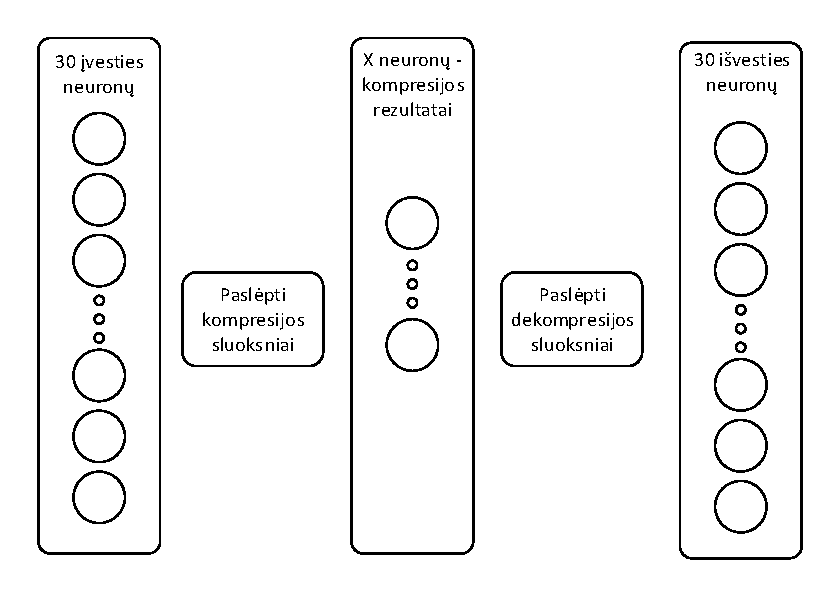
\includegraphics[scale=0.75]{diagrams/compression_perceptron}
	\caption{Dimensiškumo mažinimo perceptrono struktūra}
	\label{fig:compression_perceptron}
\end{figure}

Dimensiškumo mažinimui tyrimo metu buvo panaudotas daugiasluoksnis perceptronas (\ref{fig:compression_perceptron}~pav.).
Buvo sukurtas \cite[505~psl.]{autoencoder} straipsnyje aptariamas auto-kompresijos tinklas (angl.~\textit{autoencoder}).
Turint $N$ dimensijų ir norint jas sumažinti iki $M$, kai $M < N$, tai buvo atliekama sukūrus neuroninį tinklą, kurio pirmajame ir paskutiniajame sluoksniuose yra po $N$ neuronų, o viename iš vidinių sluoksnių - $M$ (šį vidinį sluoksnį vadinkime kompresijos sluoksniu).
Tokio neuroninio tinklo užduotis nėra tiesiog sumažinti dimensijų skaičių - tai daroma netiesiogiai.
Šiam tinklui perduodant tam tikrus $M$ dimensijų turinčius duomenis, iš jo tikimasi, kad išeities neuronuose susiformuos rezultatas, lygus pradiniams duomenims - tai yra neuronų tinklas šių duomenų nepakeis.
Ši užduotis būtų paprasta, jeigu visi vidiniai turėtų bent $N$ dimensijų - tada pateikiami duomenys galėtų būti tiesiog perkeliami iš vieno neuronų sluoksnio į kitą nepakeisti.
Tačiau kompresijos sluoksnis turi tik $M$ neuronų - vadinasi, duomenis reikės tam tikru būdu pertvarkyti, kad jie galėtų būti perduodami per šį sluoksnį prarandant kuo mažiau savybių.
Būtent čia ir įvyksta dimensiškumo mažinimas - neuroninis tinklas yra apmokomas pateikti kuo panašesnius duomenis į pradinius, o kompresijos sluoksnyje su $M$ neuronų susidaro duomenys, turintys mažiau dimensijų.
Norint sumažinti tam tikrų duomenų dimensijas, užtenka šiuos duomenis paduoti apmokytam neuroniniui tinklui ir pažiūrėti, kokie duomenys susidarė kompresijos sluoksnyje.
Nuskaičius šių neuronų reikšmes ir bus gaunami duomenys, turintis mažiau dimensijų.

Tokiame apmokytame neuroniniame tinkle visi sluoksniai, esantys kairėje nuo kompresijos sluoksnio, yra naudojami dimensiškumo mažinimui.
Būtent per šiuos sluoksnius einant signalams ir yra sudaromi mažiau dimensijų turintis duomenys.
Kadangi šio neuroninio tinklo tikslas yra pateikti rezultatą, kuris būtų kuo panašesnis į pateiktus duomenis, todėl galima teikti, kad sluoksniai, esantys dešinėje nuo kompresijos sluoksnio, yra naudojami pradinių duomenų dekompresijai.

\begin{figure}[h]
	\centering
	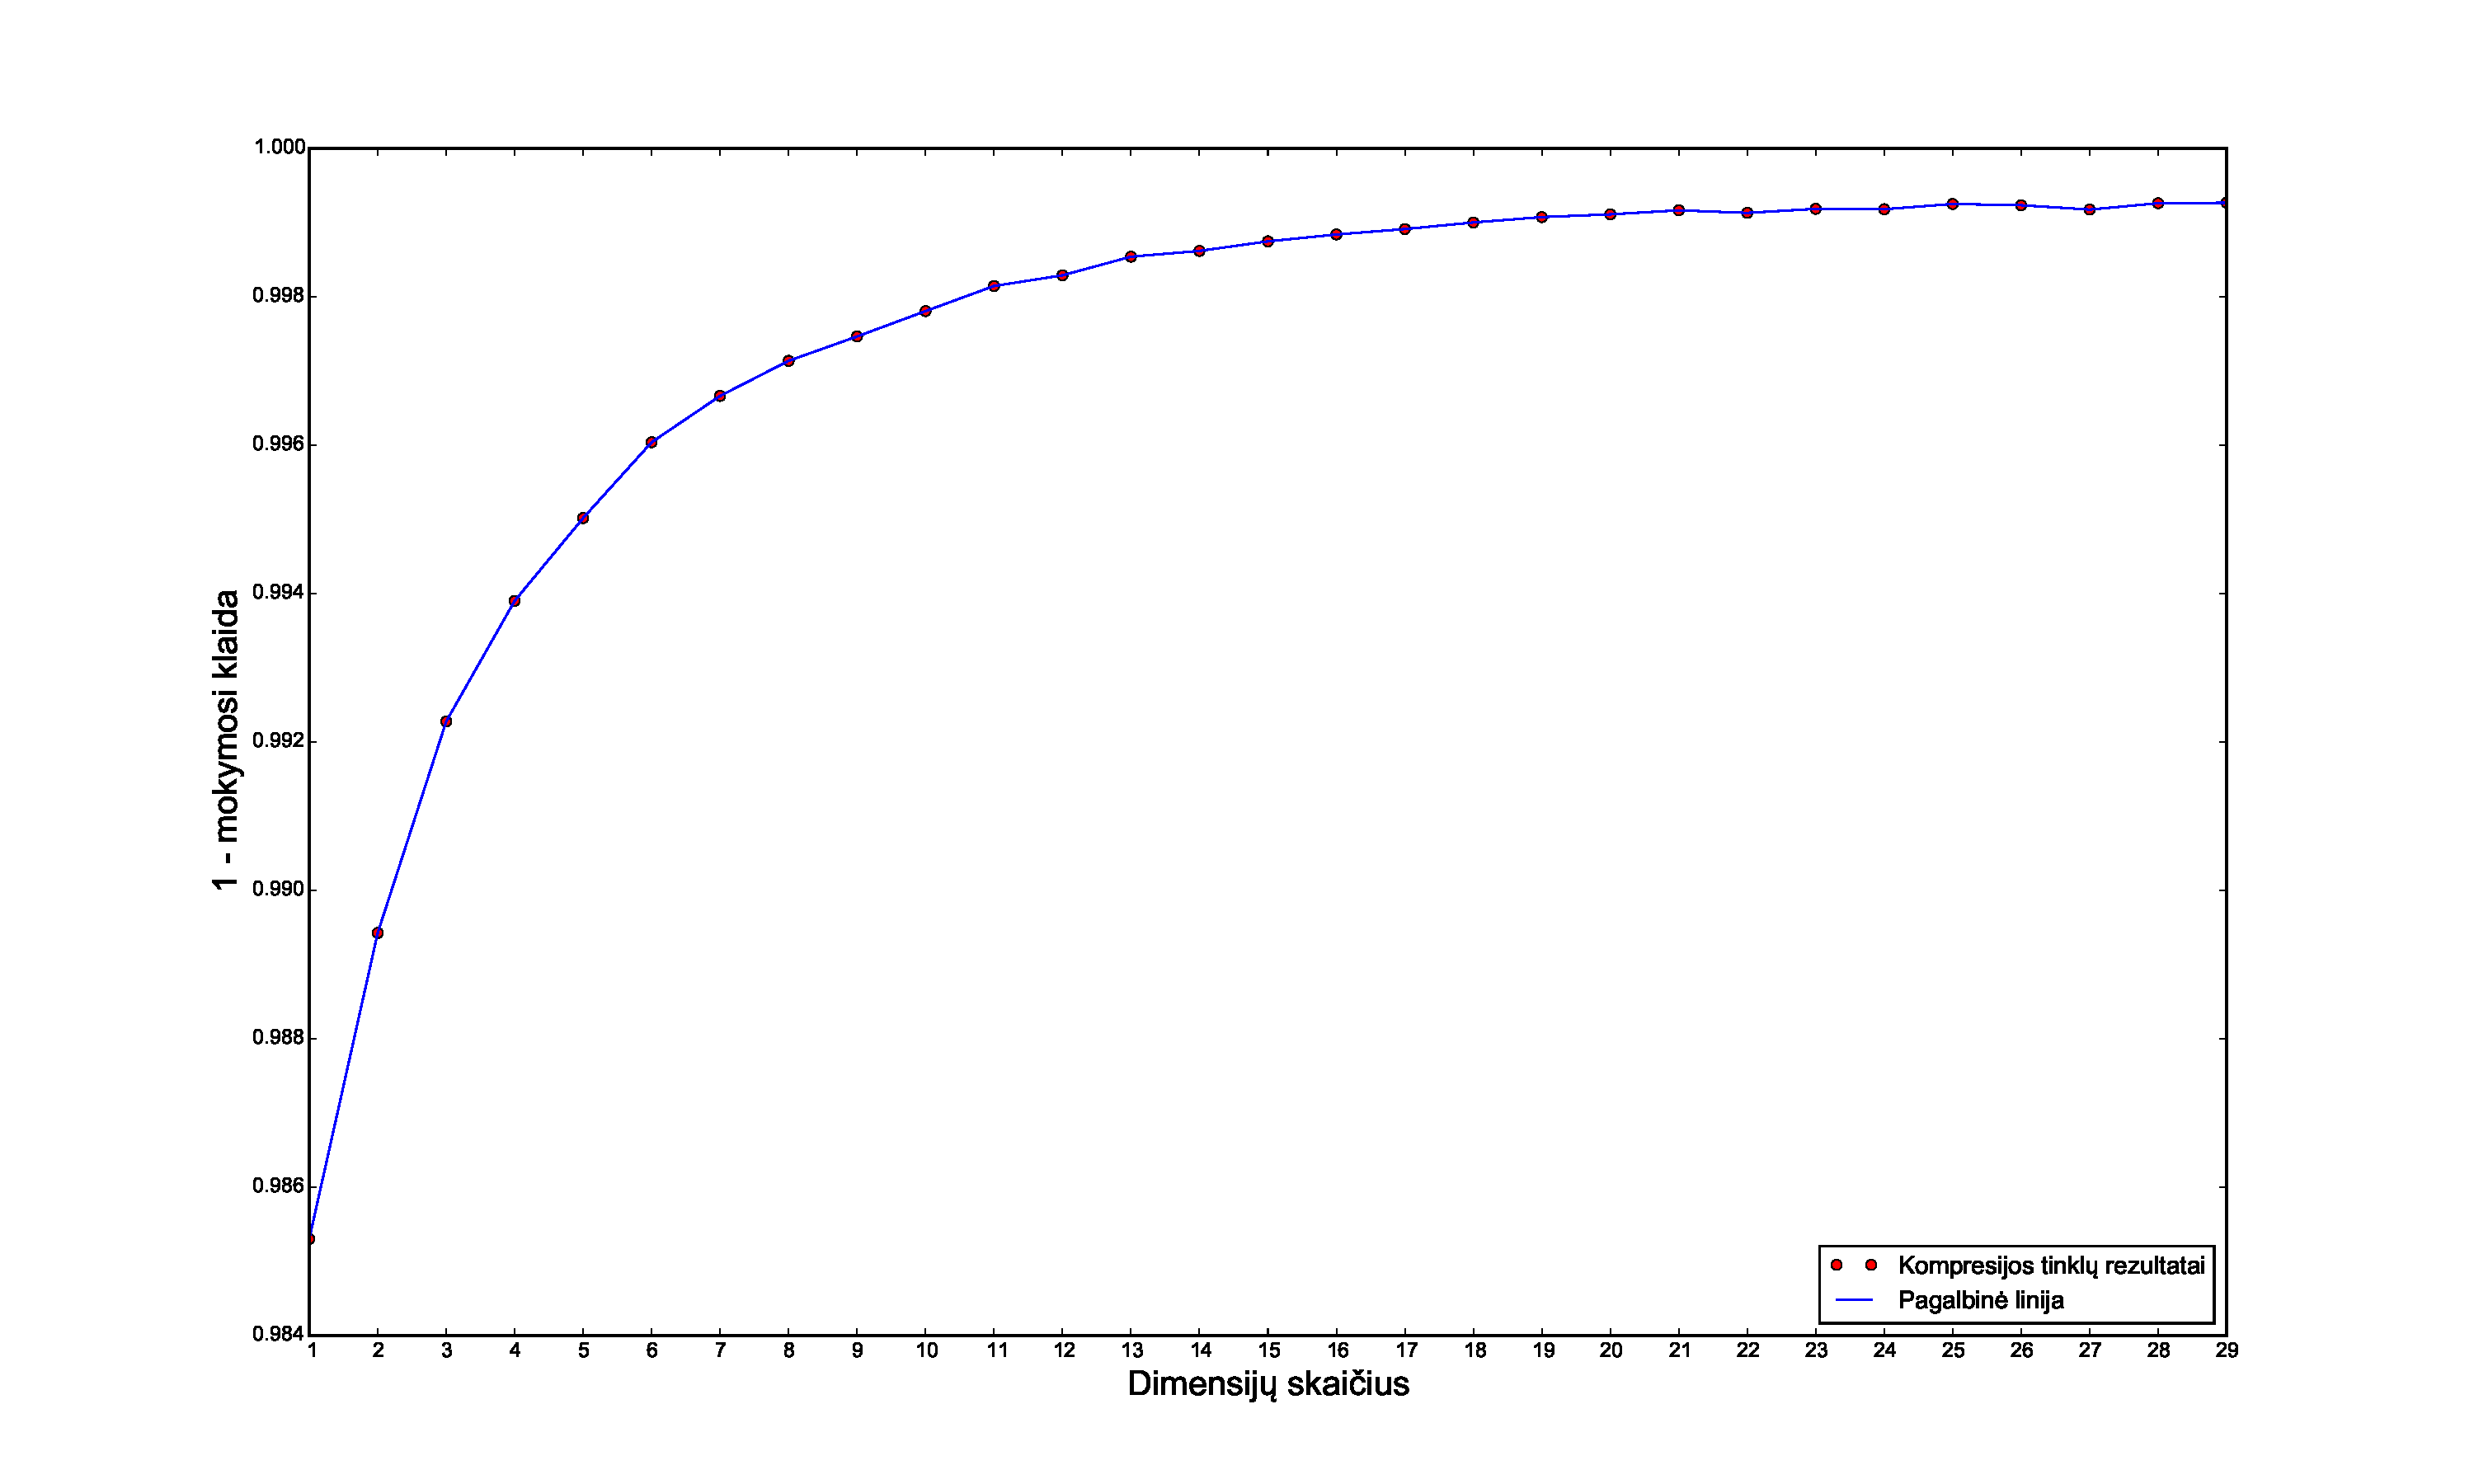
\includegraphics[scale=0.25]{pics/compression_dimensions}
	\caption{Duomenų kompresijos rezultatai}
	\label{fig:compression_dimensions}
\end{figure}

Tiriamų duomenų dimensiškumas buvo sumažintas šiuo būdu.
Dimensiškumo mažinimui buvo panaudotas daugiasluoksnis perceptronas su 5 sluoksniais - po 30 neuronų įvedimo, išvedimo ir dviejuose paslėptuose sluoksniuose, o viduriniame paslėptame sluoksnyje - tiek neuronų, į kiek dimensijų norima sumažinti duomenų dimensiškumą.
Apmokymui panaudoti $\eta = 0,2$ mokymosi bei $\mu = 0,4$ momento koeficientai.
Buvo paimta po 500 įrašų iš 3 skirtingų grupių.
Kadangi duomenys turi 30 dimensijų, duomenų dimensijos buvo mažinamos iki [1; 29] dimensijų.
Gauti rezultatai pavaizduoti \ref{fig:compression_dimensions}~pav.
Rezultatuose matoma, kaip tiksliai daugiasluoksnis kompresijos perceptronas geba atstatyti pradinius 30 dimensijų duomenis turėdamas sukompresuotus mažiau dimensijų turinčius duomenis.
Galima pastebėti, kad mažėjant dimensijų skaičiui, atstatyti pradinius duomenis darosi vis sunkiau.
Visgi mažinant dimensijų skaičių iki tam tikros ribos, kompresijos teisingumas mažėja ganėtinai lėtai.
Tęsiant dimensijų mažinimą, teisingumas pradeda kristi vis greičiau.
Iš to galima daryti prielaidą, kad analizuojamuose duomenyse yra pasikartojančios ar tiesiogiai tarpusavyje priklausančios informacijos, kurią galima sukompresuoti į mažiau dimensijų turinčią ir naudingesnę informaciją.
Tačiau svarbu pasirinkti tinkamą dimensijų skaičių, kadangi pasirinkus per mažai dimensijų, kompresija gali prarasti didelę svarbios informacijos dalį.

Pateikiami dvimačių (\ref{fig:2d_points}~pav.) ir trimačių (\ref{fig:3d_points}~pav.) duomenų kompresijos rezultatai - kairėje pusėje pavaizduoti sukompresuoti duomenys, skirtingų grupių įrašus pavaizduojant skirtingomis spalvomis, o dešinėje - tinklo apmokymo klaidos kitimo diagramos.
Iš pateiktų rezultatų matosi, kad dvimačiai duomenys susigrupavę ne taip gerai, kaip trimačiai.
Kadangi turimi duomenys turi 30 dimensijų, todėl dimensijų sumažinimas iki 2 praranda didesnę dalį duomenų nei mažinant iki 3 dimensijų.
Didesnių dimensijų kompresijos rezultatų vizualiai pavaizduoti nepavyksta dėl natūralių priežasčių.

\begin{figure}[h]
	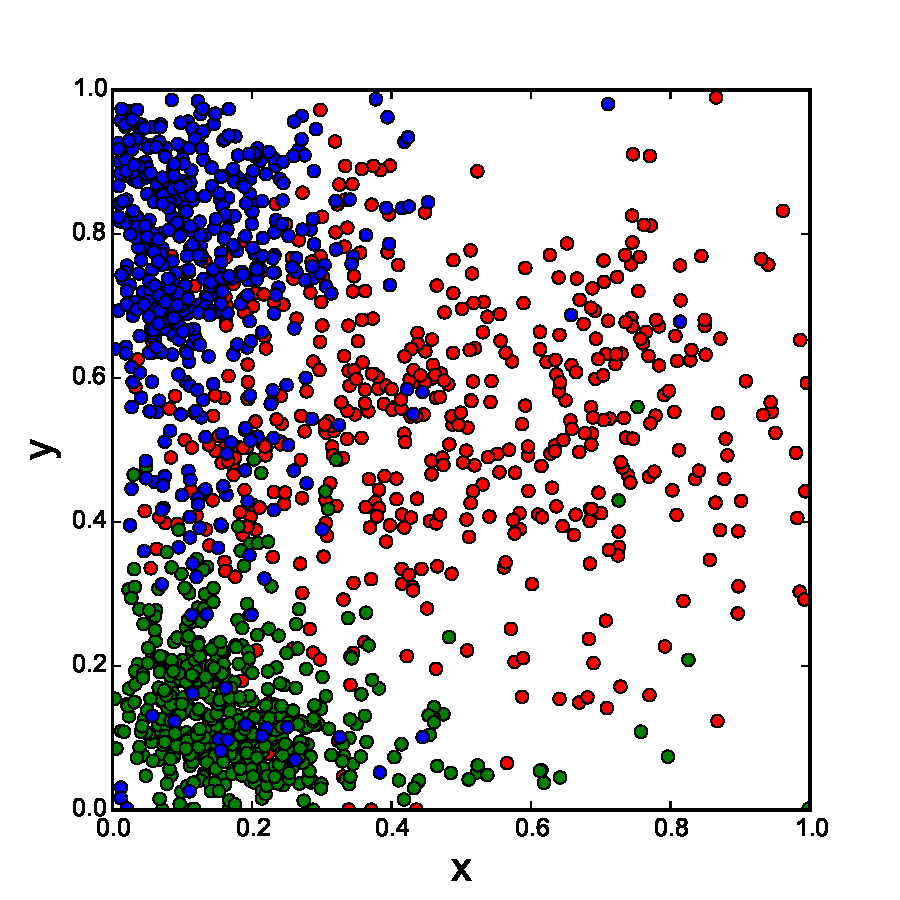
\includegraphics[scale=0.45]{pics/points_2d}
	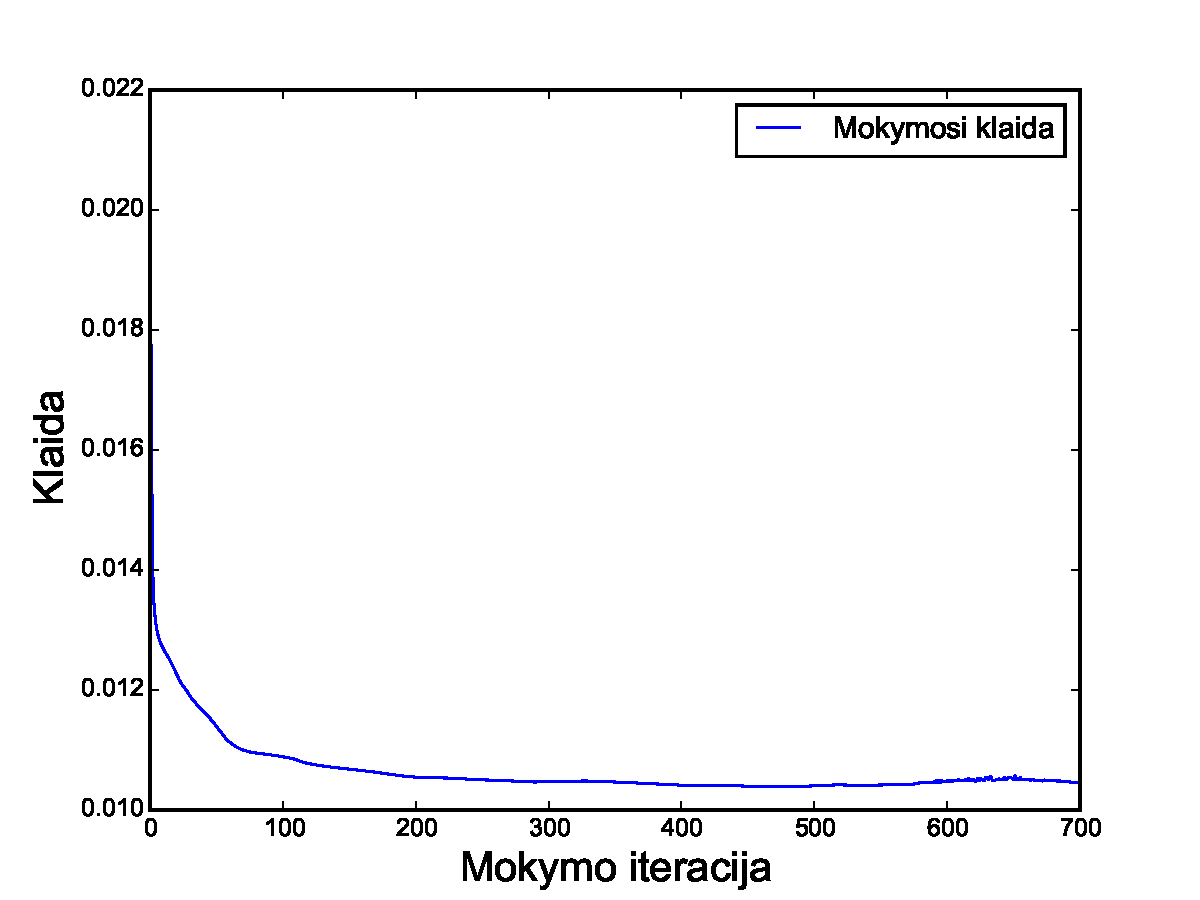
\includegraphics[scale=0.45]{pics/points_2d_progress}
	\caption{Dvimačiai duomenys}
	\label{fig:2d_points}
\end{figure}

\begin{figure}[h]
	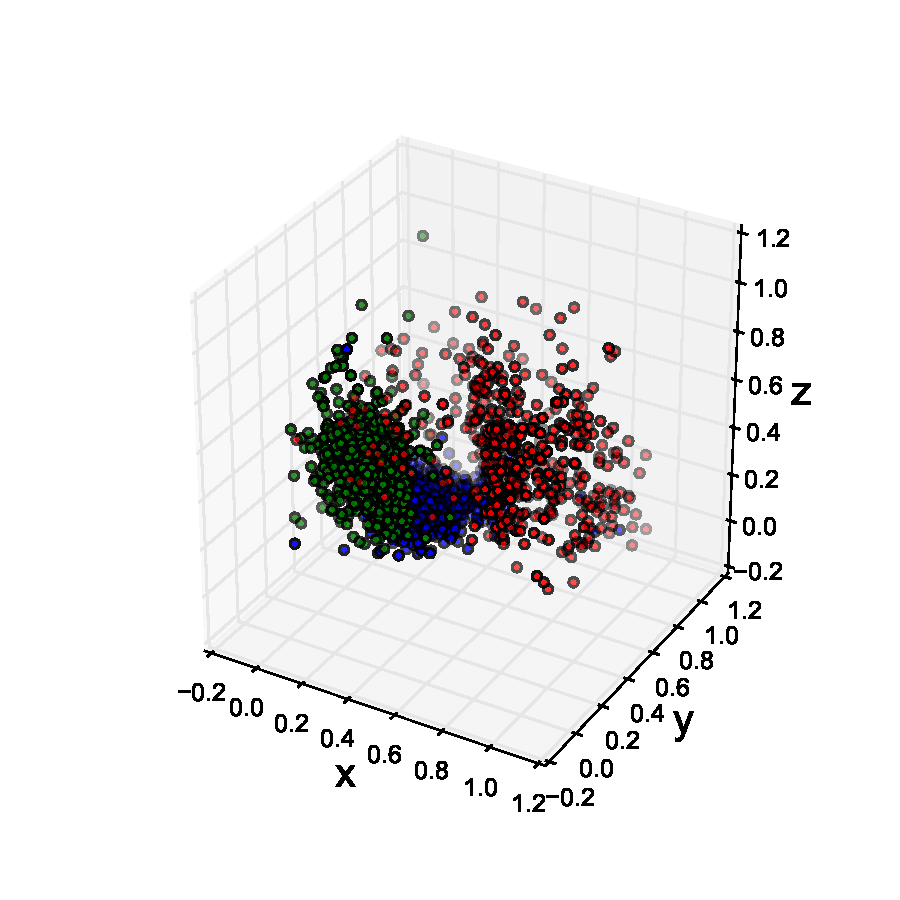
\includegraphics[scale=0.45]{pics/points_3d}
	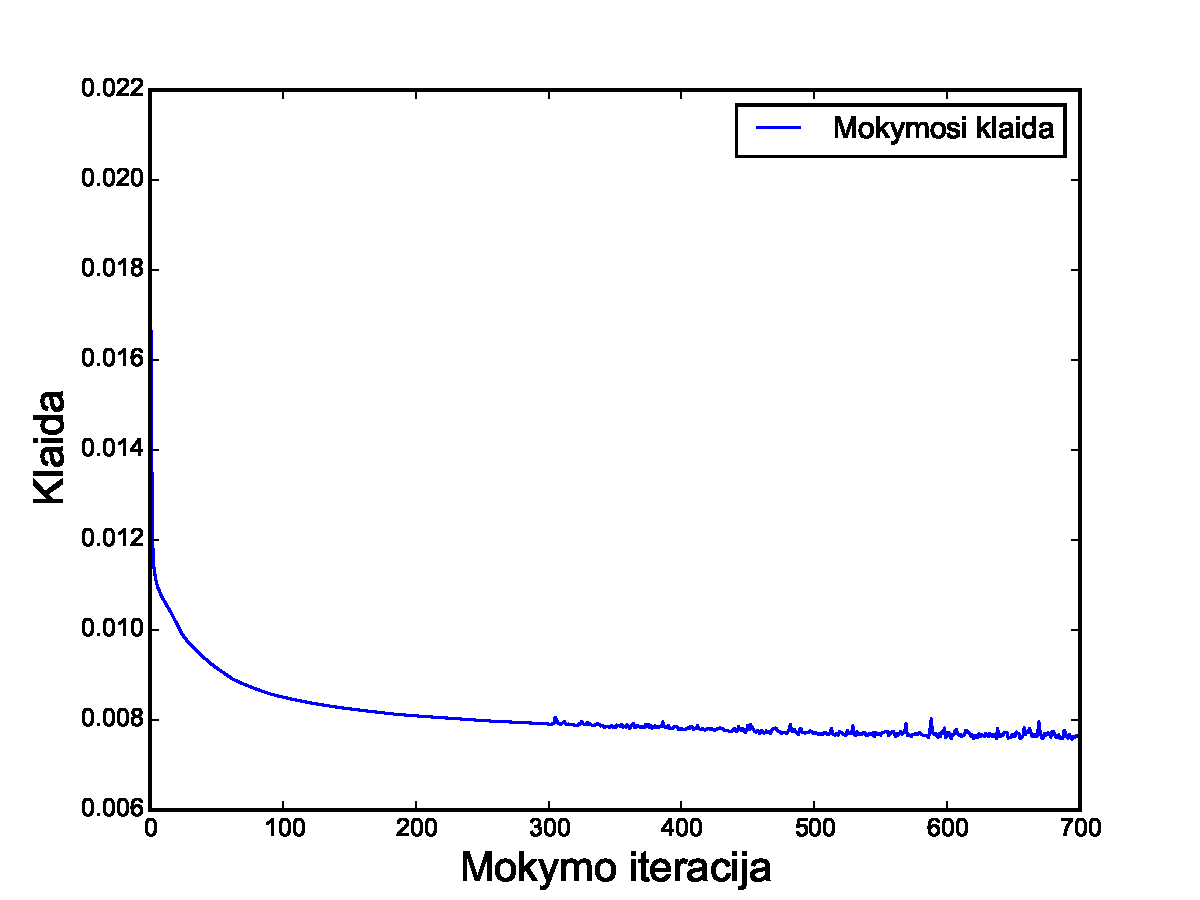
\includegraphics[scale=0.45]{pics/points_3d_progress}
	\caption{Trimačiai duomenys}
	\label{fig:3d_points}
\end{figure}



\section{Klasifikavimas mažinant dimensiškumą} \label{classification-dimensionality-reduction}

Norint išsiaiškinti, ar galima pasiekti geresnius klasifikavimo rezultatus prieš tai sumažinant duomenų dimensiškumą, buvo atliktas tyrimas.
Kadangi tiriamus duomenis sudaro 30 dimensijų, buvo bandoma sumažinti dimensijas iki visų galimų dimensijų dydžių - nuo 1 iki 29.
Norint išsiaiškinti klasifikavimo efektyvumą pasirinkus į kiek dimensijų bus kompresuojami duomenys, atliekamas eksperimentas.

Eksperimento metu pirmiausia sukuriamas ir apmokomas daugiasluoksnis perceptronas, skirtas kompresuoti duomenis į pasirinktą dimensijų skaičių.
Šį perceptroną sudaro 5 sluoksniai - įvedimo, išvedimo bei 3 paslėptieji sluoksniai.
Įvedimo, išvedimo bei 2 paslėptieji sluoksniai turi po 30 neuronų.
Trečiasis paslėptasis sluoksnis, esantys tinklo viduryje, turi tiek neuronų, į kiek dimensijų norima sukompresuoti duomenis - pagal \ref{dimensionality-reduction-perceptron} poskyryje aprašytą metodą šiame sluoksnyje ir yra gaunami sukompresuoti duomenys.
Šis sluoksnis tada yra apmokomas 300 kartų iteruojant per visus mokymo rinkinio įrašus.
Apmokius tinklą, duomenys yra sukompresuojami pasinaudojant geriausią mokymo metu pasiektą rezultatą.

Gavus sukompresuotus duomenis, pradedamas klasifikavimas.
Pirmiausia sukuriamas klasifikavimui skirtas daugiasluoksnis perceptronas.
Šį perceptroną sudaro 4 sluoksniai.
Pirmasis - įvesties sluoksnis, turintis tiek neuronų, kiek dimensijų turi sukompresuoti duomenys.
Tada du paslėpti sluoksniai, turintys po 30 neuronų.
Galiausiai, išvesties sluoksnis, turintis tiek neuronų, kiek yra skirtingų galimų klasių.
Kadangi šio eksperimento metu buvo analizuojami duomenys iš 3 skirtingų klasių, todėl išvesties sluoksnis turėjo 3 neuronus.
Šis tinklas buvo apmokomas panaudojant iš kompresijos tinklo gautais kompresuotais duomenimis.
Apmokymui buvo naudojami $\eta = 0,2$ mokymosi bei $\mu = 0,4$ momento koeficientai.
Apmokymas vyko 400 kartų, kaskart mokymo metu panaudojant visus mokymo rinkinio įrašus.
Baigus apmokymą, gaunamas rezultatas - klasifikavimo klaida.

Kiekvienam galimam dimensijų skaičiui, į kurį norima sutraukti duomenis, šis eksperimentas buvo atliktas po kelis kartus.
Taip buvo užtikrinama, kad gauti rezultatai bus patikimesni, kadangi kai kuriais atvejais atsitiktinai sugeneruoto perceptrono struktūra gali būti labai nepalanki ir gali būti gaunamas prastas rezultatas, neparodantis, kiek visgi toks kompresijos mažinimas gali padėti klasifikavimui.



\subsection{Sumažinto dimensiškumo duomenų klasifikavimo perceptronų galimybių eksperimentas}

Pirmiausia šis eksperimentas buvo atliktas su daliniais duomenimis.
Iš kiekvienos grupės paimta po 50 įrašų, kurie buvo naudojami eksperimentuose tiek apmokymui, tiek ir pačiam tinklo klaidos skaičiavimui.
Taip buvo pasielgta norint išsiaiškinti perceptronų galimybes - kadangi visi duomenys, kurie naudojami klaidos skaičiavime, yra naudojami taip pat ir apmokant, neuroniniui tinklui nelieka nežinomų duomenų.
Pirmiausia šie duomenys buvo panaudoti apmokant kompresijos tinklą, kuris po to buvo panaudotas šiems duomenims sukompresuoti.
Tada šie sumažinto dimensiškumo duomenys buvo panaudoti klasifikavimo tinklo apmokymui.
Apmokius klasifikavimo tinklą, gaunama klaida.
Tai atlikus po 5 kartus visiems galimiems dimensijų skaičiams, gauti rezultatai, pavaizduoti \ref{fig:experiment-1}~pav.
Raudoni taškai žymi visų klasifikavimo apmokymų rezultatus, o mėlyna linija išryškina visų dimensijų geriausius apmokymo rezultatus.

\begin{figure}[h]
	\centering
	\centerline{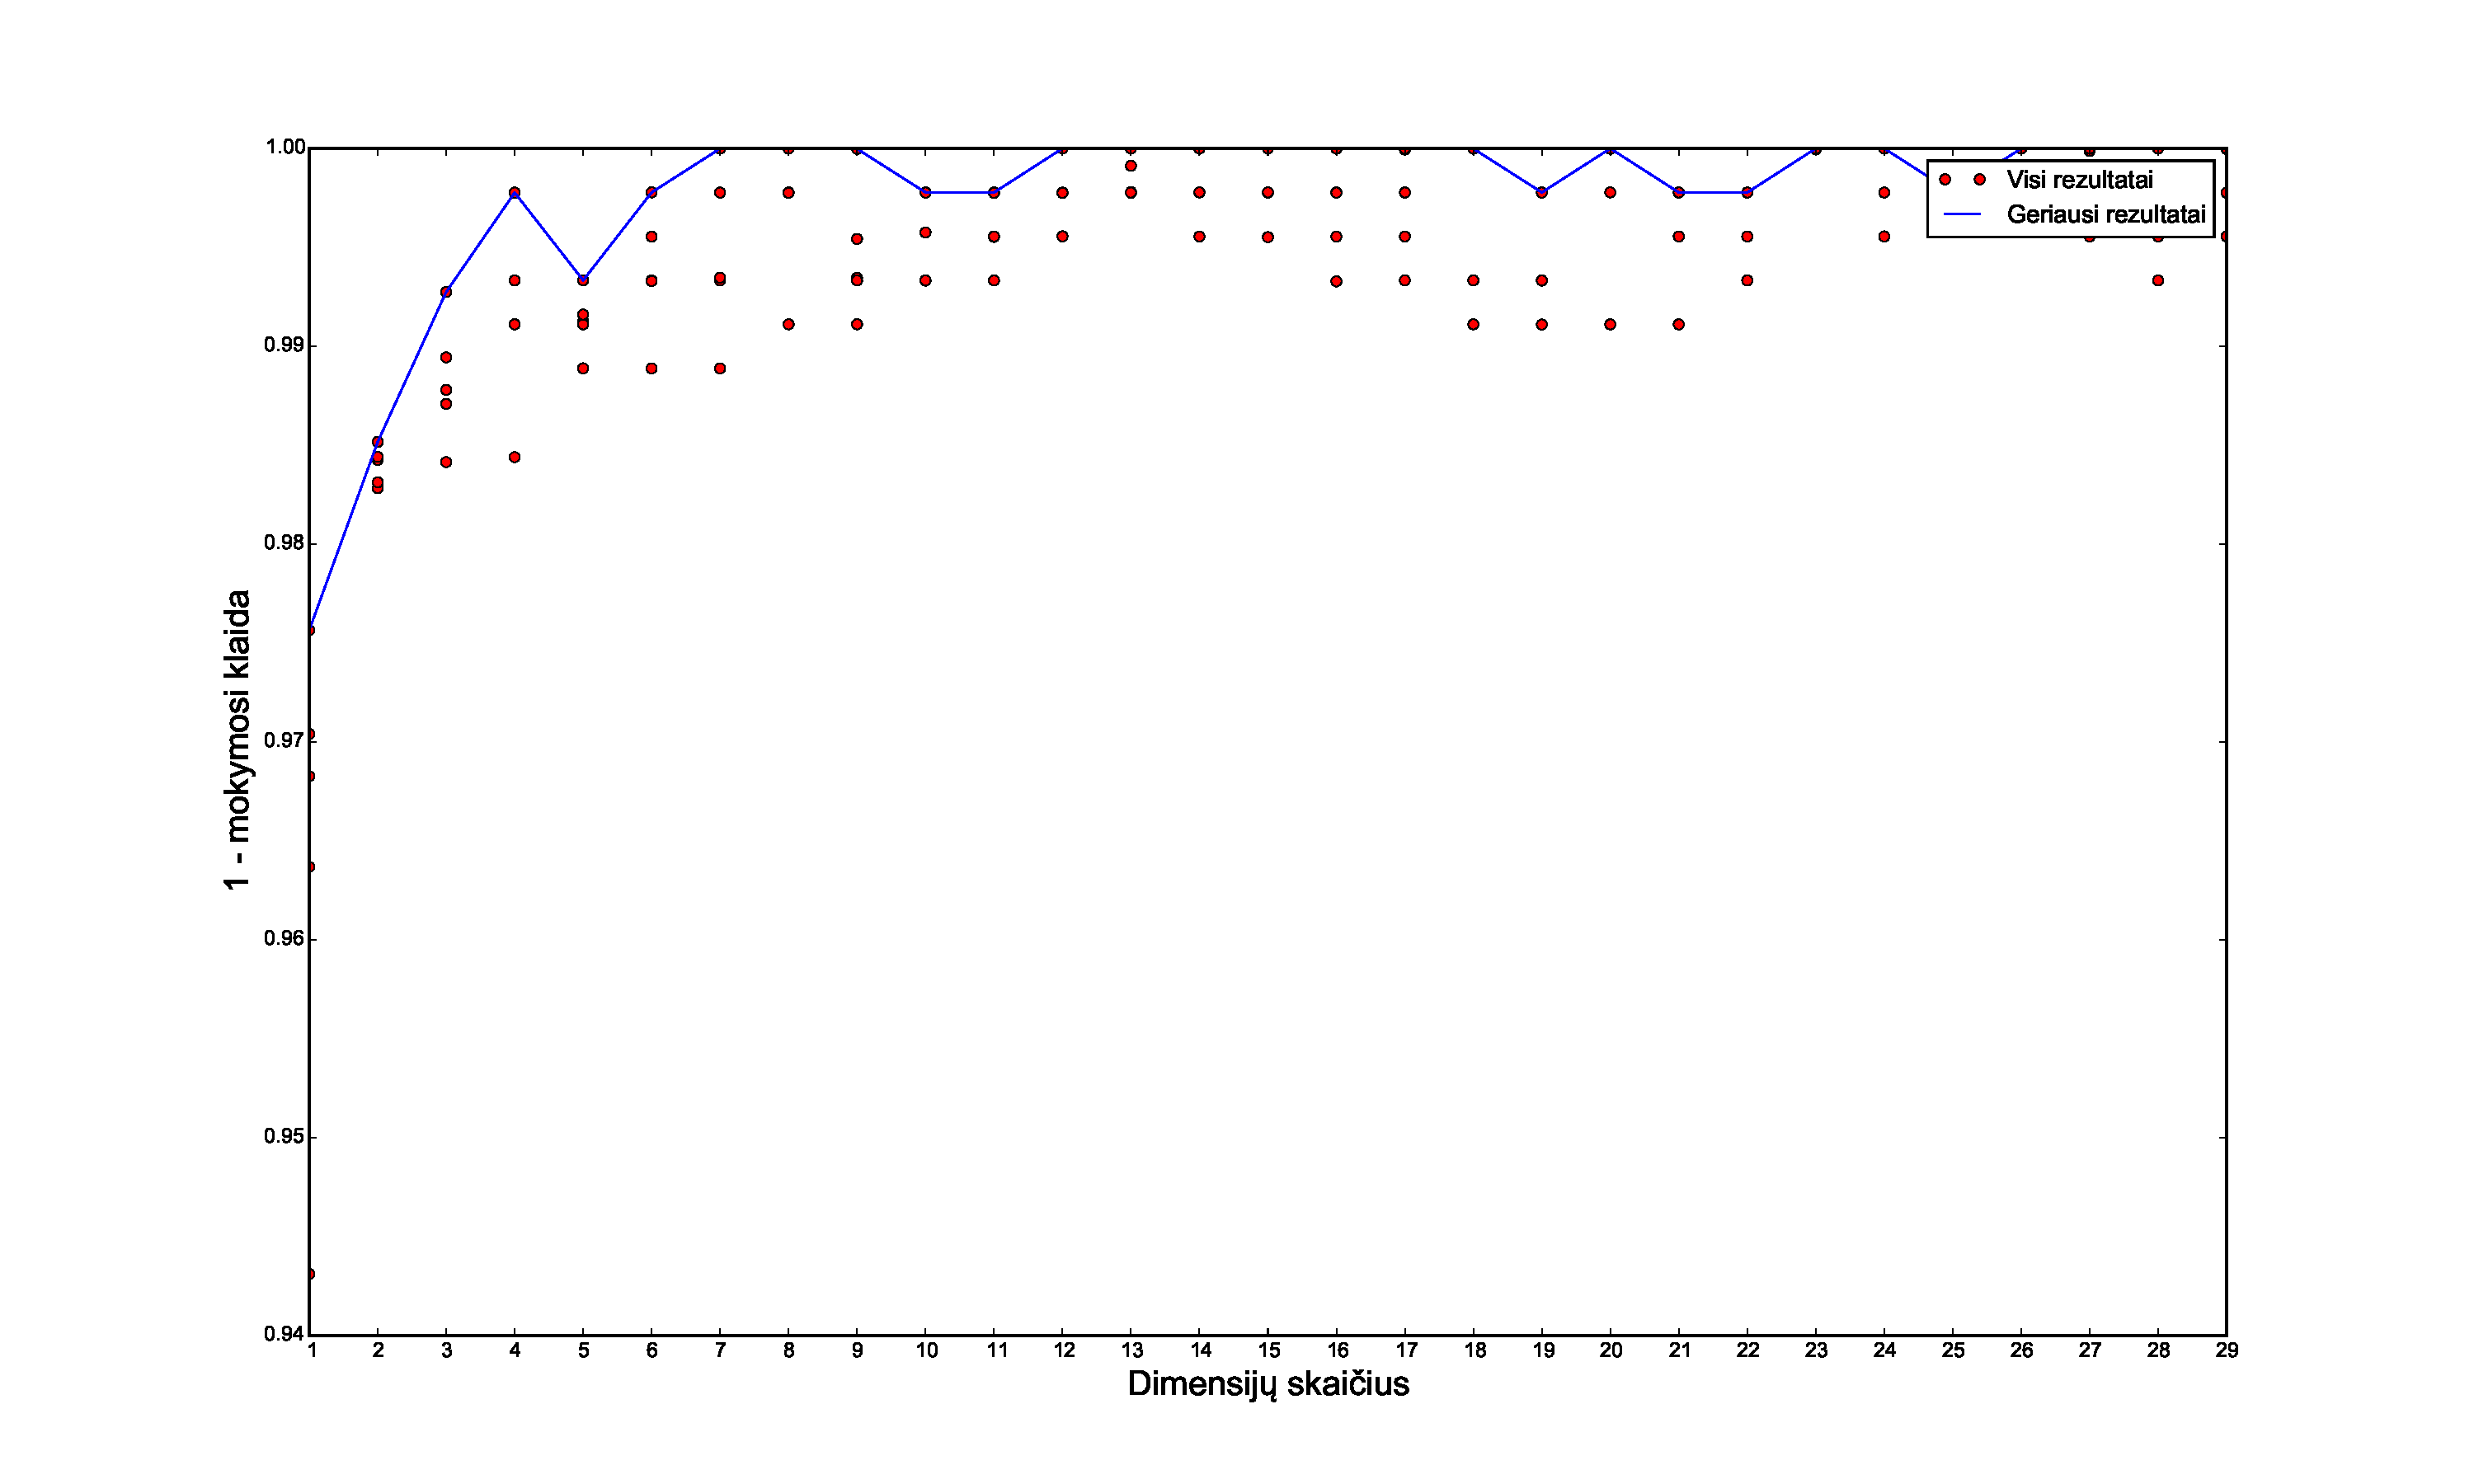
\includegraphics[scale=0.37]{pics/dimensions_2015-5-23_15-50-6}}
	\caption{Klasifikavimo mažinant dimensijas rezultatai}
	\label{fig:experiment-1}
\end{figure}

Iš rezultatų matosi, kad klasifikavimo tinklas gerai geba susidoroti su tokiais mažais duomenimis - rezultatai labai netoli vieneto, tai yra, klaida beveik lygi nuliui.
Išimtis tyrimuose su mažais dimensijų skaičiais - kai dimensijų yra mažai, neuronų tinklas nesugeba suklasifikuoti sukompresuotų duomenų.
Tai parodo, kad mažinant dimensijų skaičių iki labai mažo, prarandama dalis informacijos apie duomenis.
Dėl to juos klasifikuoti pasidaro sunkiau.
Todėl norint padidinti klasifikavimo efektyvumą, dimensijų skaičių galima mažinti daugiausiai iki keturių.



\subsection{Kompresuotų duomenų klasifikavimo eksperimentas}

Sekančiame atliktame eksperimente buvo panaudoti visi įrašai iš tiriamų grupių - 500 įrašų iš 3 grupių.
Kompresijos perceptrono apmokymui buvo panaudoti visi šie įrašai, kadangi tikslas yra kuo tiksliau ir autentiškiau sukompresuoti visus duomenis, o ne paruošti tinklą, kuris gebėtų kompresuoti dar tinklui nematytus duomenis.
Apmokius kompresijos tinklą, gaunami kompresuoti duomenys.
Tada iš kiekvienos grupės atsitiktinai pasirenkama po 50 įrašų, kurie naudojami klasifikavimo perceptrono apmokymui.
Apmokius perceptroną, jo klaida skaičiuojama su visais duomenimis, o ne tik naudotais mokymo metu.
Taip dauguma įrašų perceptronui yra nauji, todėl taip ištiriama, kaip gerai perceptronas sugebėjo išmokti duomenų savybes iš mažų mokymo grupių.
Eksperimentas buvo atliktas kiekvienam dimensijų skaičiui po 30 kartų, norint užtikrinti kuo mažesnį atsitiktinumą.
Gauti rezultatai, pavaizduoti \ref{fig:experiment-2}~pav.
Raudoni taškai žymi visų klasifikavimo validacijų rezultatus, o mėlyna linija išryškina visų dimensijų geriausius validacijos rezultatus.

Iš šių rezultatų matosi, kad su pakankamai mažais dimensijų skaičiais (mažesniais nei 13), klasifikavimo perceptronas gauna šiek tiek didesnę klaidą nei su likusiais dimensijų skaičiais.
Taip turbūt atsitinka dėl panašių priežasčių, kaip ir pirmame tyrime su dimensijų skaičiais nuo vieno iki trijų - kompresija praranda dalį svarbios duomenų informacijos.
To nesimato pirmame eksperimente, kadangi skirtumai gan maži - blogiausias tyrimas pasiektas su 5 dimensijomis, kurio metu gauta klaida apie $1 - 0,965 = 0,035$.
Tuo tarpu praeitame eksperimente, kuriame buvo ištirti dar mažesni dimensijų skaičiai, blogiausias tyrimas pasiektas su viena dimensija, kurio klaida apie $1 - 0,943 = 0,057$ beveik dvigubai didesnė.
Tai didelis skirtumas žinant, kad pirmame eksperimente klaidos skaičiavimui buvo naudojami visi apmokymui naudoti duomenys.
Geriausi rezultatai gauti $[14; 29]$ dimensijų skaičiaus intervale.
Šio eksperimento metu patikimiausiai atrodo rezultatai su 18 dimensijų, todėl šis dimensijų skaičius buvo pasirinktas palyginimui.

\begin{figure}[h]
	\centering
	\centerline{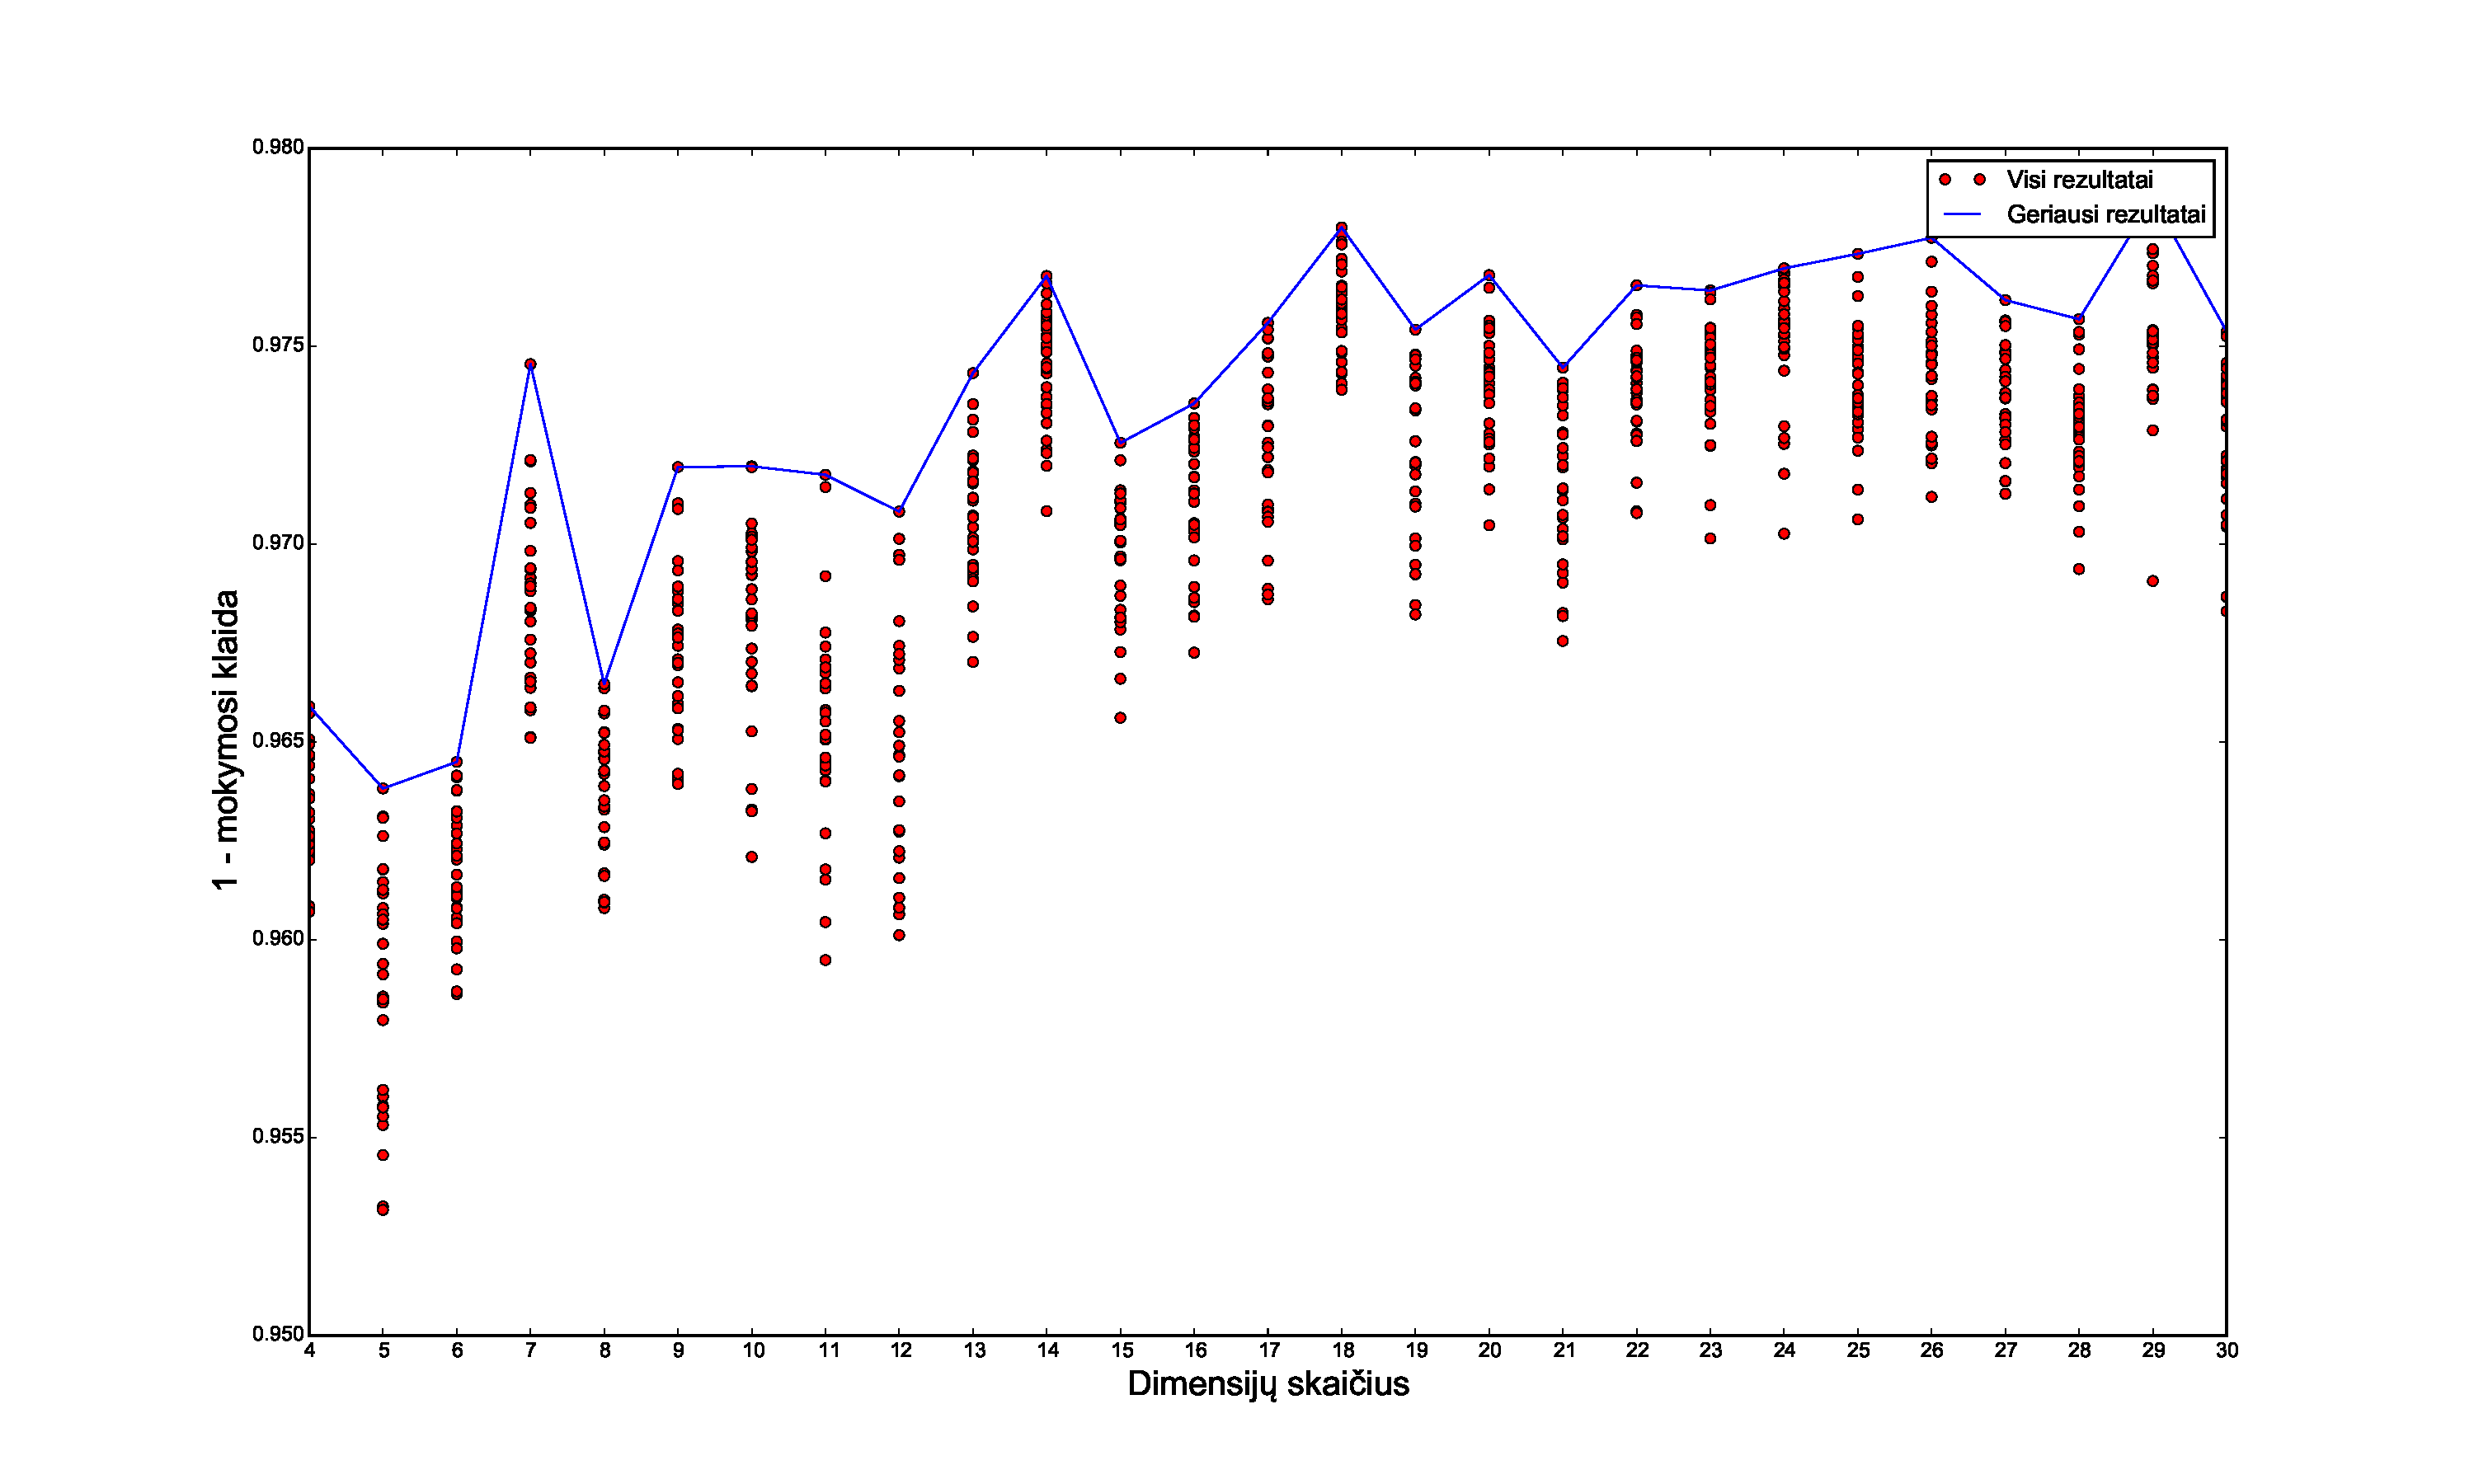
\includegraphics[scale=0.37]{pics/dimensions_2015-5-27_6-18-5}}
	\caption{Klasifikavimo mažinant dimensijas rezultatai}
	\label{fig:experiment-2}
\end{figure}


\subsection{Originalių ir sumažinto dimensiškumo duomenų klasifikavimo palyginimas}

Buvo atliktas klasifikavimo efektyvumo palyginimas naudojant originalius 30-ties dimensijų bei kompresuotus 18-os dimensijų duomenis.
Palyginimui buvo naudojami tie patys duomenys - po 500 įrašų iš kiekvienos grupės, ir tik po 50 iš jų naudojami apmokymui (validacijai buvo panaudoti visi 500 įrašų iš kiekvienos grupės).
Gautas rezultatai pavaizduotas \ref{fig:dim-comparisons}~pav.

\begin{figure}[H]
	\centering
	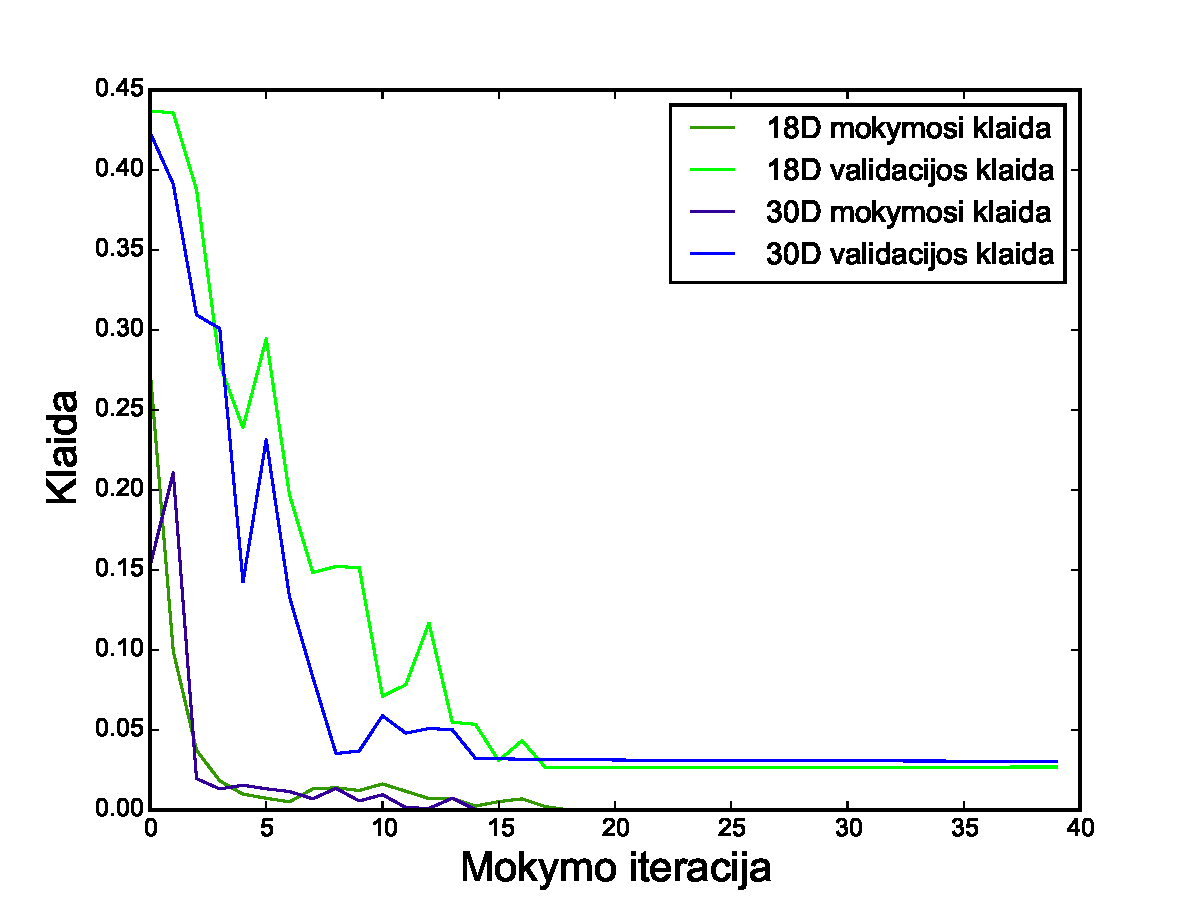
\includegraphics[scale=0.8]{pics/dim_comparisons_2015-5-27_14-21-13}
	\caption{18 ir 30 dimensijų klasifikavimo apmokymų palyginimas}
	\label{fig:dim-comparisons}
\end{figure}

Iš rezultatų matosi, kad abu daugiasluoksniai klasifikavimo perceptronai sugebėjo pasiekti beveik nulinę klaidą mokymo procese.
Tai reiškia, kad tinklai pilnai išmoko mokymui naudotus duomenis ir daugiau pastebimai tobulėti negali.
Visgi galutinė validacijos klaida skiriasi - 18-os dimensijų duomenų validacijos klaida mažesnė už 30-ties.

Taip pat buvo atliktas bandymas, kurio metu buvo skaičiuojama, kiek duomenų daugiasluoksniai klasifikavimo perceptronai suklasifikavo teisingai.
Buvo sukurta, apmokyta ir ištestuota po 100 tinklų kompresuotiems 18-os dimensijų bei originaliems 30-ies dimensijų duomenims.
Daugiasluoksnių perceptronų, analizuojančių originalius 30-ies dimensijų duomenis, teisingai suklasifikuotų atvejų skaičius buvo intervale $[1413, 1443]$.
Tuo tarpu 18 dimensijų analizuojančių - intervale $[1427, 1449]$.
Šie rezultatai detaliau pavaizduoti \ref{fig:correct-count}~pav.

\begin{figure}[h]
	\centering
	\centerline{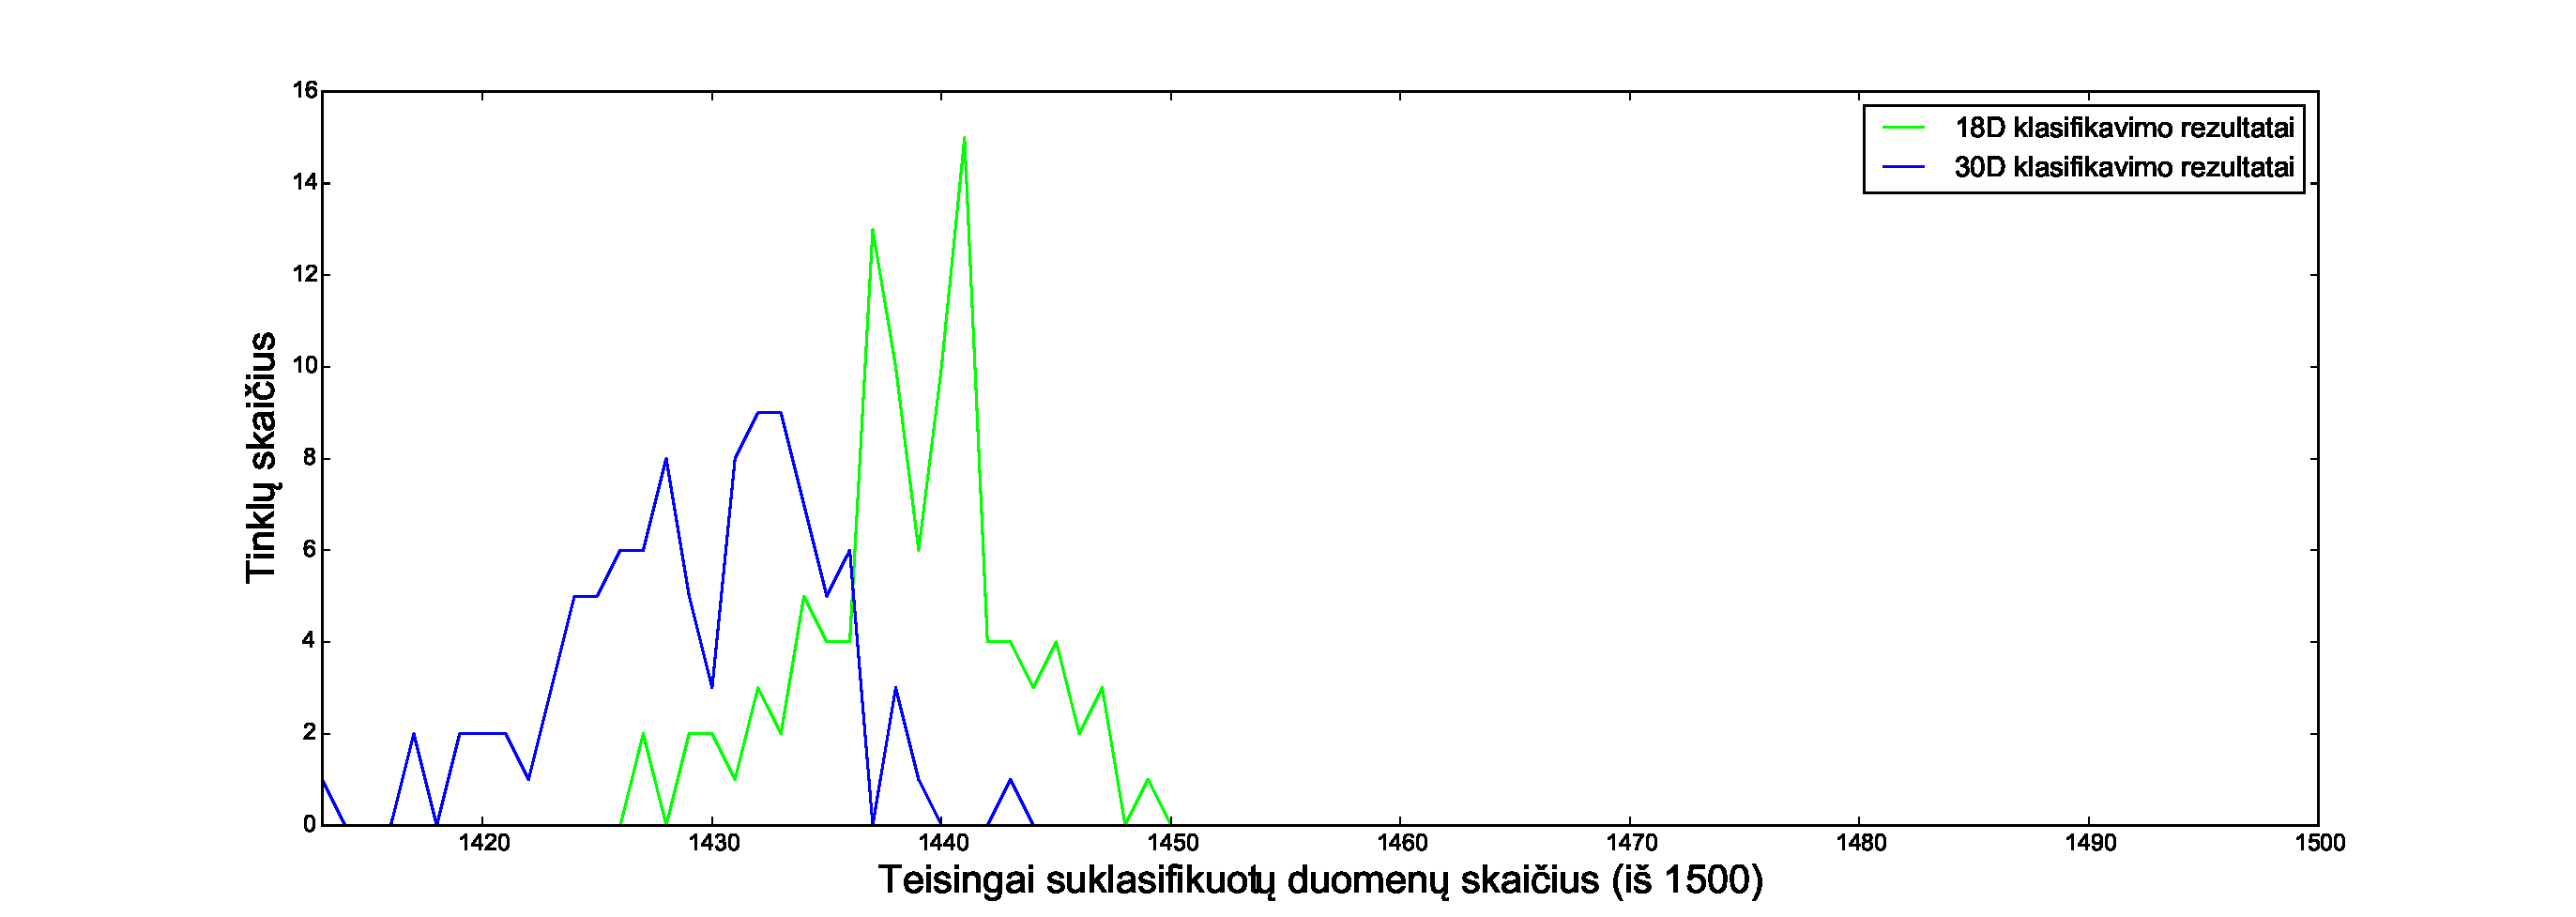
\includegraphics[scale=0.43]{pics/correct}}
	\caption{18 ir 30 dimensijų klasifikavimo rezultatų palyginimas}
	\label{fig:correct-count}
\end{figure}

Apskaičiuota, kad vidutinis teisingai suklasifikuotų duomenų skaičius 30-ies dimensijų tinkluose apytiksliai lygus $1429,4$, o 18-os dimensijų - apytiksliai $1438,6$.
Kadangi iš viso buvo 1500 klasifikavimui naudotų duomenų, todėl 30-ies dimensijų tinklai blogai klasifikavo vidutiniškai apie 70.6 duomenų (apie $4.70\%$ visų duomenų), o 18-os dimensijų - vidutiniškai apie 61.4 duomenų (apie $4.09\%$ visų duomenų).
Tai reiškia, kad dimensiškumo mažinimas vidutiniškai sumažino apie $(70.6 - 61.4) / 70.6 = 13.03\%$ visų padarytų klaidų.



\sectionnonum{Rezultatai ir išvados}

Šio darbo metu pasiekti rezultatai:
\begin{enumerate}
	\item Suprogramuotas daugiasluoksnis perceptronas.
	\item Suprojektuotas ir suprogramuotas klasifikuojantis daugiasluoksnis perceptronas.
	\item Klasifikuojantis daugiasluoksnis perceptronas ištestuotas su tam parinktais vilkdalgių duomenimis.

	\item Peržvelgti keli dimensiškumo mažinimo metodai bei išanalizuota tiesinė diskriminantinė analizė bei dimensiškumo mažinimas daugiasluoksniu perceptronu.
	\item Tyrimui pasirinktas dimensiškumo mažinimo daugiasluoksniu perceptronu metodas.
	\item Suprojektuotas ir suprogramuotas dimensiškumo mažinimo daugiasluoksnis perceptronas.
	\item Tiriamų chromosomų duomenų dimensiškumas sumažintas iki visų galimų dimensijų skaičių, ištirta dimensiškumo mažinimo įtaka duomenims sumažinto dimensiškumo duomenis bandant atstatyti į pradinius.

	\item Atlikti tyrimai, analizuojantys, kaip keičiasi klasifikavimo rezultatas mažinant daugiasluoksniui perceptronui perduodamų duomenų dimensiškumą.
	\item Pasirinktas optimalus dimensiškumo mažinimui naudojamas dimensijų skaičius.
	
	\item Palygintos daugiasluoksnių perceptronų apmokymo bei validacijos klaidos naudojant sumažinto ir nesumažinto dimensiškumo duomenis.
	\item Palyginti sumažinto ir nesumažinto dimensiškumo duomenų klasifikavimo rezultatai.
\end{enumerate}

Išvados:
\begin{enumerate}
	\item Tiriamųjų duomenų dimensiškumą galima mažinti neprarandant daug informacijos, jeigu dimensijų skaičius nesumažinamas per stipriai.
	\item Kuo didesniu skaičiumi mažinamos tiriamų duomenų dimensijos, tuo daugiau informacijos prarandama, ir vis didinant šį skaičių, prarandamos informacijos kiekis vis labiau auga.
	\item Mažinant duomenų dimensiškumą, svarbu parinkti ne per mažą dimensijų skaičių, nes priešingu atveju duomenys gali prarasti svarbią dalį informacijos.
	\item Nustatyta, kad klasifikavimą galima pagerinti sumažinant klasifikavimui naudojamų duomenų dimensiškumą.
	\item Norint pagerinti tiriamų duomenų klasifikavimą, jų dimensijų skaičių verta sumažinti iki daugumos intervalo $[14; 29]$ skaičių.
	\item Ištirta, kad vienas optimaliausių dimensiškumo mažinimui naudojamų dimensijų skaičių yra 18.

	\item Tiek su sumažinto, tiek ir su nesumažinto dimensiškumo duomenimis daugiasluoksnių perceptronų apmokymo klaidos beveik pasiekia nulį. Tuo tarpu validacijos klaidos truputį didesnės, naudojant sumažinto dimensiškumo duomenis validacijos klaida šiek tiek mažesnė. Vadinasi, abiem atvejais mokymui naudoti duomenys buvo gerai įsisavinti, tačiau bendri rezultatai geresni naudojant sumažinto dimensiškumo duomenis.
	\item Tiriamų duomenų dimensijų skaičių sumažinus iki 18, klaidų skaičius vidutiniškai sumažėja apie $13.03\%$.
\end{enumerate}



\printbibliography[heading=bibintoc]  % Šaltinių sąraše nurodoma panaudota
% literatūra, kitokie šaltiniai. Abėcėlės tvarka išdėstomi darbe panaudotų
% (cituotų, perfrazuotų ar bent paminėtų) mokslo leidinių, kitokių publikacijų
% bibliografiniai aprašai. Šaltinių sąrašas spausdinamas iš naujo puslapio.
% Aprašai pateikiami netransliteruoti. Šaltinių sąraše negali būti tokių
% šaltinių, kurie nebuvo paminėti tekste. Šaltinių sąraše rekomenduojame
% necituoti savo kursinio darbo, nes tai nėra oficialus literatūros šaltinis.
% Jei tokių nuorodų reikia, pateikti jas tekste.

% \sectionnonum{Sutartinis terminų žodynas}
% Sąvokų apibrėžimai ir santrumpų sąrašas sudaromas tada, kai darbo tekste
% vartojami specialūs paaiškinimo reikalaujantys terminai ir rečiau sutinkamos
% santrumpos.

\end{document}
